\documentclass{article}
\usepackage[utf8]{inputenc}
\usepackage{amssymb}
\usepackage{amsthm}
\usepackage{enumerate}
\usepackage{pgfplots}
\usepackage{mathtools}
\usepackage{nicefrac}
\usepackage{centernot}
\usepackage{fourier}
\usepackage{tikz}
\usepackage[inline,shortlabels]{enumitem}
\usepackage{hyperref}
\usepackage{imakeidx}
\usepackage{thmtools}
\usepackage[framemethod=TikZ]{mdframed} % Needed for the box and shading
\usepackage{xcolor} % To define custom colors

\definecolor{lightgray}{gray}{0.9}


\title{Analysis on the Real Line}
\author{Cam Quilici - Instructor Dr. Andrea Bonito}
\date{Fall 2023}

\setlist[itemize,1]{topsep=0pt,itemsep=2em,partopsep=0.5em,parsep=0pt}

\newcommand{\Z}{\mathbb{Z}}
\newcommand{\C}{\mathbb{C}}
\newcommand{\Q}{\mathbb{Q}}
\newcommand{\R}{\mathbb{R}}
\newcommand{\N}{\mathbb{N}}
\newcommand{\seq}[2]{(#1_{#2})_{#2 \in \N}}
\newcommand{\sseq}[3]{(#1_{#2_#3})_{#3 \in \N}}
\newcommand{\set}[2]{\{ #1 \mid #2 \}}
\newcommand{\sg}[1]{\langle#1\rangle}
\newcommand{\mylim}[2]{\lim_{#1 \to #2}}
\newcommand{\mylimmm}[2]{\lim\limits_{#1 \to #2}}
\newcommand{\bigslant}[2]{{\raisebox{.2em}{$#1$}\left/\raisebox{-.2em}{$#2$}\right.}}
\newcommand{\?}{\stackrel{?}{=}}
\def\checkmark{\tikz\fill[scale=0.4](0,.35) -- (.25,0) -- (1,.7) -- (.25,.15) -- cycle;}
\newcommand{\smallblacksquare}{\rule{0.5em}{0.5em}}
\newcommand\encircle[1]{%
  \tikz[baseline=(X.base)] 
    \node (X) [draw, shape=circle, inner sep=0] {\strut #1};}

\DeclareMathOperator{\ord}{ord}
\DeclareMathOperator{\norm}{Nm}

\makeatletter
\renewcommand\thmt@listnumwidth{4.3em}
\makeatother

\newmdtheoremenv[
    nobreak=true,
    backgroundcolor=lightgray,
    skipabove=1em,
    innertopmargin=.5em, % space added at the top
    innerbottommargin=1em, % space added at the bottom
    innerleftmargin=1em, % space added on the left
    innerrightmargin=1em, % space added on the right
]{theorem}{Theorem}[subsection]
\newmdtheoremenv[
    nobreak=true,
    skipabove=1em,
    innertopmargin=.5em, % space added at the top
    innerbottommargin=1em, % space added at the bottom
    innerleftmargin=1em, % space added on the left
    innerrightmargin=1em, % space added on the right
]{lemma}[theorem]{Lemma} % shares counter with theorem
\newmdtheoremenv[
    nobreak=true,
    skipabove=1em,
    innertopmargin=.5em, % space added at the top
    innerbottommargin=1em, % space added at the bottom
    innerleftmargin=1em, % space added on the left
    innerrightmargin=1em, % space added on the right
]{proposition}{Proposition}[subsection] % Proposition environment

\theoremstyle{definition} % This style is typically used for definitions, examples, etc.
\newtheorem{definition}[subsection]{Definition} % Numbered by subsection

\makeindex

\begin{document}

\maketitle

\vspace{-0.3in}
\noindent
\rule{\linewidth}{0.4pt}

\tableofcontents

\newpage

\section{The Real Numbers}

\subsection{Introduction}

\begin{itemize}
    \item[]
          \begin{lemma}
              The equation $x^2 - 2 = 0$ has no solution in $\Q$.
              \index{Lemma \thelemma}
          \end{lemma}
          \begin{proof}
              By contradiction, assume there exists some $\nicefrac{p}{q} \in \Q$, $p, q \in \N$, $q \neq 0$ such that
              $$\left(\frac{p}{q}\right)^2 - 2 = 0. \quad (*)$$
              Without loss of generality, we can assume that the greatest common divisor between $p$ and $q$ is 1. We rewrite (*) as $p^2 = 2q^2$ which implies that $p^2$ is even. This means that $p$ is even as well.
          \end{proof}
    \item We say that $\N$ is well-ordered, but not $\Q$ since $\Q$ does not have a least element.
    \item[]
          \begin{proposition}
              There is no natural number such that $0 < n < 1$.
          \end{proposition}
          \begin{proof}
              Left as an exercise.
          \end{proof}
\end{itemize}

\subsubsection{Axioms of the Real Numbers}

\begin{itemize}
    \item Binary operations:
          \begin{itemize}[label=$\smallblacksquare$]
              \item ($+$): $\R \times \R \mapsto \R \qquad x, y \in \R, \ x + y \in \R$,
              \item ($\cdot$): $\R \times \R \mapsto \R \qquad x, y \in \R, \ x \cdot y \in \R$.
          \end{itemize}
    \item We have axioms for the real numbers as follows:
          \begin{enumerate}[label=\Roman*]
              \item Algebraic Axioms
                    \begin{enumerate}[label=(\roman*)]
                        \item Associativity: For $x, y, z \in \R$, we have
                              \begin{align*}
                                  x + (y + z)         & = (x + y) + z         \\
                                  x \cdot (y \cdot z) & = (x \cdot y) \cdot z
                              \end{align*}
                        \item Commutativity: For $x, y \in \R$, we have
                              \begin{align*}
                                  x + y     & = y + x     \\
                                  x \cdot y & = y \cdot x
                              \end{align*}
                        \item Distributivity: For $x, y, z \in \R$, we have
                              \begin{align*}
                                  x \cdot (y + z) & = x \cdot y + x \cdot z
                              \end{align*}
                        \item Identity:
                              \begin{itemize}[label=$\smallblacksquare$]
                                  \item Addition: There exists some $0 \in \R$ such that for all $x \in \R$, $x + 0 = x$.
                                  \item Multiplication: There exists some $1 \in \R$ such that for all $x \in \R$, $x \cdot 1 = x$.
                              \end{itemize}
                        \item Inverses:
                              \begin{itemize}[label=$\smallblacksquare$]
                                  \item Addition: For all $x \in \R$, there exists some $y \in \R$ such that
                                        $$x + y = 0 \iff y = -x.$$
                                  \item Multiplication: For all $x \in \R$, there exists some $y \in \R$ such that
                                        $$x \cdot y = 1 \iff y = \frac{1}{x} \iff y = x^{-1}.$$
                              \end{itemize}
                    \end{enumerate}
              \item Ordering
                    \begin{enumerate}[label=(\roman*)]
                        \item For some $x, y, z \in \R$, we have
                              $$x \leq y \implies x + z \leq y + z.$$
                        \item For some $x, y \in \R$, we have
                              $$0 \leq x, 0 \leq y \implies 0 \leq x \cdot y.$$
                        \item For some $x, y, z \in \R$, we have
                              $$x \leq y, y \leq z \implies x \leq z.$$
                        \item For some $x, y \in \R$, we have
                              $$x \leq y, y \leq x \implies x = y.$$
                        \item For some $x, y \in \R$, we have
                              $$x \neq y \implies x \leq y \text{ or } y \leq x.$$
                    \end{enumerate}
              \item No Hole (not satisfied by $\Q$) \\
                    For any non-empty subset $X$ of $\{x > 0\}$, there exists some $a \in \R$ such that
                    \begin{enumerate}[label=(\arabic*)]
                        \item $a \leq x \ \forall x \in X$, and
                        \item For all $\varepsilon > 0 (\varepsilon \neq 0, 0 \leq \varepsilon)$, there exists some $x_\varepsilon$ such that $x_\varepsilon - a \leq \varepsilon$.
                    \end{enumerate}
          \end{enumerate}
\end{itemize}

\subsubsection{Bounded Intervals}

\begin{itemize}
    \item Given $a < b$, the set $X$ of real numbers is a bounded interval if it is in the form:
          \begin{itemize}[label=\smallblacksquare]
              \item Open interval with endpoints $a, b$
                    $$\set{x \in X}{a < x < b} = (a, b).$$
              \item Closed intervals
                    $$\set{x \in X}{a \leq x \leq b} = [a, b].$$
              \item Half-open intervals
                    $$\set{x \in X}{a < x \leq b} = (a, b].$$
          \end{itemize}
\end{itemize}

\subsection{Supremum and Infimum}

\begin{itemize}
    \item[]
          \begin{definition}[Boundedness]
              Let $X \subseteq \R$ be non-empty. A number $m \in \R$ (not necessarily in $X$) is a \textbf{lower bound} for $X$ if for all $x \in X$, $m \leq x$.
          \end{definition}
          If a set has a lower bound, it is called \textbf{bounded below} (for instance, $\Z$).
    \item \textbf{Remark}. $X$ either has no lower bounds or infinitely many.
    \item[]
          \begin{definition}[Infimum]
              Let $X \subseteq \R$ be non-empty. A number $s \in \R$ (not necessarily in $X$) is called an \textbf{infimum} of the set $X$ if it is
              \begin{enumerate}[label=(\arabic*)]
                  \item A lower bound and
                  \item For all other lower bounds $r_i$ of $X$, $s \geq r_i$.
              \end{enumerate}
              The infimum is hence known as the ``greatest lower bound." We denote ``$r$ is the infimum of $X$" as
              $$r = \inf(X).$$
          \end{definition}
    \item[]
          \begin{definition}[Supremum]
              Let $X \subseteq \R$ be non-empty. A number $s \in \R$ (not necessarily in $X$) is called a \textbf{supremum} of the set $X$ if it is
              \begin{enumerate}[label=(\arabic*)]
                  \item An upper bound and
                  \item For all other upper bounds $r_i$ of $X$, $s \leq r_i$.
              \end{enumerate}
              The supremum is hence known as the ``least upper bound." We denote ``$r$ is the supremum of $X$" as
              $$r = \sup(X).$$
          \end{definition}
    \item[]
          \begin{theorem}
              Let $X \subseteq \R$ be non-empty. $X$ has an upper bound if and only if $X$ has a finite supremum and the finite supremum is unique.
          \end{theorem}
          \begin{proof}
              If $X$ has a supremum then that supremum is an upper bound for $X$. Assume that $b$ is an upper bound of $X$. Let $\overline{X} = \set{b + 1 - y}{y \in X}$, then $\overline{X}$ is non empty and $\overline{X} \subset \{x > 0\}$ (there is a 1 so it is surely greater than 0). \\\\
              So, by Axiom 3, there is a real number $a$ such that
              \begin{enumerate}[label=(\arabic*)]
                  \item If $z \in \overline{X}$, then $a \leq z$ (i.e., $a$ is a lower bound for $\overline{X}$) and
                  \item For every $\varepsilon > 0$, there exists a $z_\varepsilon \in \overline{X}$ such that
                        $$z_\varepsilon - a \leq \varepsilon.$$
              \end{enumerate}
              \textbf{Claim}. $b_1 = b + 1 - a$ is the supremum for $X$. \\\\
              There are two things to check:
              \begin{enumerate}[label=(\arabic*)]
                  \item Is $b_1$ an upper bound for $X$? Well, if $y \in X$, then $a \leq b + 1 - y$ and we have $y \leq b + 1 - a = b_1$.
                  \item Is $b_1$ the least upper bound? \\\\
                        Let $M$ be some upper bound for $X$. Let us show that $b_1 \leq M$. By way of contradiction, assume that $M < b_1 = b + 1 - a$. Let $\varepsilon = b_1 - M > 0$. \\\\
                        By Axiom 3, there exists some $z \in \overline{X}$ such that $z - a \leq \varepsilon$. We have
                        $$z = b + 1 - y, y \in X, \qquad \varepsilon = b_1 - M = b + 1 - a - M.$$
                        So, supposedly $z - a = b + 1 - y - a \leq b + 1 - a - M$ with $M \leq y$ (this is a contradiction since $M$ is assumed to be an upper bound, it cannot be smaller than $y$) and therefore $b_1 \leq M$ and $b_1 = \sup(X)$.
              \end{enumerate}
          \end{proof}
    \item \textbf{Archimedean Axiom} (satisfied in $\R$). For every $x > 0, y \geq 0$, there exists $n \in \N_*$ such that
          $$n \cdot x > y.$$
          \begin{proof}
              By way of contradiction, assume that $n \cdot x \leq y \ \forall n \in \N_*$ (for some $x > 0, y \geq 0)$. Then let $S = \set{n \cdot x}{n \in \N_*} \subset \R$. Clearly $S$ is bounded above by $y$ and $S$ is non-empty. This implies that $\sup(S)$ exists and $n \cdot x \leq \sup(s) \ \forall n \in \N_*$. This all implies that $(m + 1) \cdot x \leq \sup(S) \ \forall m \in \N_*$
          \end{proof}
    \item[]
          \begin{lemma}
              Let $X \subset \R$ be non-empty and bounded above. Then for every $\varepsilon > 0$, there exists some $x_\varepsilon$ such that
              $$\sup(X) - \varepsilon < x_\varepsilon \leq \sup(X).$$
          \end{lemma}
          \begin{proof}
              Since $\sup(X)$ is an upper bound for $X$, then we know $x \leq \sup(X) \ \forall x \in X$. This implies the second part of the inequality. \\\\
              To prove the first part of the inequality, assume by way of contradiction that there exists some $\varepsilon_0 > 0$ such that for every $x \in X$, $\sup(x) - \varepsilon_0 \geq x$. However, this is not possible since $\sup(x)$ is an upper bound, i.e., subtract anything from it and it will be less than $x$.
          \end{proof}
    \item[]
          \begin{lemma}
              Let $x, y \in \R$ with $y > x$, then there exists some $r \in \Q$ such that $x < r < y$.
          \end{lemma}
          \begin{proof}
              Take $y - x > 0$, the Archimidean principle guarantees the existence of $n \in \N$ such that
              $$n \cdot (y - x) > 1 \iff y - x > \frac{1}{n}.$$
              Recall,
              \begin{align*}
                  \lfloor x \rfloor  & \leq x \leq \rfloor x \lfloor + 1     \\
                  \lfloor nx \rfloor & \leq \frac{nx}{n} < \frac{nx + 1}{n}.
              \end{align*}
              Let $r := \nicefrac{(\lfloor nx \rfloor + 1)}{n} \in \Q$. Then we have
              \begin{align*}
                  x = \frac{nx}{n} & < \frac{\lfloor nx \rfloor + 1}{n} \\
                                   & \leq \frac{nx + 1}{n}              \\
                                   & = x + \frac{1}{n}                  \\
                                   & = x + y - x                        \\
                                   & < y.
              \end{align*}
          \end{proof}
    \item \textbf{Corollary.} Let $p, q \in \Q$ with $p < q$. There exists some $z \in \R \ \symbol{92} \ \Q$ such that $p < z < q$.
          \begin{proof}
              By Lemma,
              \begin{align*}
                  \frac{p}{c} < \frac{q}{c} & \iff \frac{p}{c} < \underbrace{r}_{\in \Q} < \frac{q}{c}         \\
                                            & \iff p < \underbrace{r \cdot c}_{\in \R \ \symbol{92} \ \Q} < q.
              \end{align*}
          \end{proof}
\end{itemize}

\subsubsection{Absolute Value}

\begin{itemize}
    \item[]
          \begin{definition}[Absolute value]
              For some $x \in \R$, the \textbf{absolute value} function is defined as follows:
              \[ |x| := \begin{cases}
                      -x & \text{, if } x < 0     \\
                      x  & \text{, if } x \geq 0.
                  \end{cases} \]
          \end{definition}
    \item[]
          \begin{proposition}
              Let $x, a \in \R$. Then we have
              \begin{enumerate}[label=(\roman*)]
                  \item $|x| = 0 \iff x = 0$.
                  \item Let $a > 0$, then
                        \begin{itemize}[label=\smallblacksquare]
                            \item $|x| < a \iff -a < x < a$
                        \end{itemize}
              \end{enumerate}
          \end{proposition}
\end{itemize}

\section{Sequences}

\subsection{Convergence}

\begin{itemize}
    \item[]
          \begin{definition}[Sequential convergence]
              A sequence of real numbers $\seq{x}{n}$ is said to be \textbf{convergent} if there exists $x \in \R$ such that $\forall \varepsilon > 0 \ \exists N(\varepsilon) \in \N$ such that
              $$|x - x_n| \leq \varepsilon \ \forall n \geq N(\varepsilon).$$
              Furthermore, we write $\lim_{n \to \infty} x_n = x$.
          \end{definition}
    \item \textbf{Example}. Show that $\lim_{n \to \infty} 1 + \nicefrac{1}{(n + 1)} = 1$. We want
          $$|x - x_n| = \left|1 - \left(1 + \frac{1}{n + 1}\right)\right| = \left|\frac{1}{n + 1}\right| = \frac{1}{n + 1} \leq \varepsilon \ \forall \varepsilon > 0.$$
          Let $\varepsilon > 0$, set $N(\varepsilon) = \lfloor \nicefrac{1}{\varepsilon} \rfloor = N(\varepsilon)$. This holds for
          \begin{align*}
              |x - x_n| & = \frac{1}{n + 1} \leq \frac{1}{\lfloor \frac{1}{\varepsilon} \rfloor + 1} \\
                        & \leq \frac{1}{\frac{1}{\varepsilon}} \leq \varepsilon.
          \end{align*}
    \item[]
          \begin{lemma}
              A sequence of real numbers has \textbf{at most} one limit.
          \end{lemma}
          \begin{proof}
              Assume $l_1, l_2 \in \R$ are two limits. We will show that $l_1 = l_2$ by showing that for all $\varepsilon > 0$, $|l_1 - l_2| \leq \varepsilon$. Let $\varepsilon > 0$.
              \begin{enumerate}[label=(\arabic*)]
                  \item $\seq{x}{n}$ converges to $l_1$, i.e., for all $\varepsilon_1 > 0 \ \exists N_1(\varepsilon_1)$ such that
                        $$|x_n - l_1| \leq \varepsilon_1 \ \forall n \geq N_1(\varepsilon_1),$$
                  \item $\seq{x}{n}$ converges to $l_2$, i.e., for all $\varepsilon_2 > 0 \ \exists N_2(\varepsilon_2)$ such that
                        $$|x_n - l_2| \leq \varepsilon_2 \ \forall n \geq N_2(\varepsilon_2).$$
              \end{enumerate}
              Let $\varepsilon > 0$ and set $\varepsilon_1 - \nicefrac{\varepsilon}{2}, \varepsilon_2 = \nicefrac{\varepsilon}{2}$. Then we have
              \begin{align*}
                  |l_1 - l_2| & = |l_1 - x_n + x_n - l_2|                       \\
                              & \leq |l_1 - x_n| + |l_2 - x_n| \leq \varepsilon
              \end{align*}
              where $|l_1 - x_n| \leq \varepsilon_1 \ \forall n \geq N_1$ and $|l_2 - x_n| \leq \varepsilon_2 \  n \geq N_2 \ n \geq \max\{N_1, N_2\}$. Altogether, this implies that $l_1 = l_2$.
          \end{proof}
    \item \textbf{Example of Divergent Sequence}. Take $x_n = n \cdot \sin(n \cdot \nicefrac{\pi}{2})$. By way of contradiction, assume that $\seq{x}{n}$ is converging to some $x \in \R$. Say
          \begin{align*}
              x_{p_n} & = x_{4n + 1} = (4n + 1) \cdot \underbrace{\sin((4n + 1) \cdot \frac{\pi}{2})}_{= 1} \\
                      & = 4n + 1                                                                            \\
              x_{q_n} & = x_{4n + 5} = (4n + 5) \cdot \underbrace{\sin((4n + 5) \cdot \frac{\pi}{2})}_{= 1} \\
                      & = 4n + 5
          \end{align*}
          which implies that $|x_{p_n} - x_{x_n}| = 4$. From the contradiction assumption, for $\varepsilon = \nicefrac{1}{2}$ there exists $N(\nicefrac{1}{2})$ such that
          $$|x_n - x| \leq \frac{1}{2} \ \forall n \geq N(\frac{1}{2}).$$
          Take $n$ such that $4n + 1 \geq N(\nicefrac{1}{2})$. Then we have
          \begin{align*}
              |x_{p_n} - x| & \leq \frac{1}{2}                                    \\
              |x_{q_n} - x| & \leq \frac{1}{2}                                    \\
              4             & = |x_{p_n} - x_{q_n}| = |x_{p_n} - x + x - x_{q_n}| \\
                            & \leq |x_{p_n} - x| + |x_{q_n} - x|                  \\
                            & \leq \frac{1}{2} + \frac{1}{2} \leq 1
          \end{align*}
          but this is a contradiction, so $\seq{x}{n}$ must be divergent.
    \item[]
          \begin{lemma}
              Every convergent sequence is bounded.
          \end{lemma}
          \begin{proof}
              Let $\seq{x}{n}$ be a convergent sequence, that is, there exists some $x \in \R$ such that for all $\varepsilon > 0$, there exists some $N(\varepsilon) \in \N$ and
              $$|x - x_n| \leq \varepsilon \ \forall n \geq N(\varepsilon).$$
              In particular, take for $\varepsilon = 1$, there is $N(1)$ such that
              $$|x_n - x| \leq 1 \ \forall n \geq N(1).$$
              Recall the reverse triangle inequality,
              \begin{alignat*}{2}
                  |x_n| - |x|       & \leq |x - x_n|     &  & \leq 1 \quad n \geq N(1) \\
                  \implies \, |x_n| & \leq 1 + |x| \quad &  & n \geq N(1)
              \end{alignat*}
              Let $M = \max\{|x_0|, |x_1|, \ldots, |x_{N(1) - 1}|, 1 + |x|\}$. Then certainly
              \begin{align*}
                  |x_n|          & \leq M \qquad n \leq N(1)       \\
                  |x_n|          & \leq M \qquad n \geq N(1)       \\
                  \implies |x_n| & \leq M \qquad \forall n \in \N.
              \end{align*}
          \end{proof}
    \item \textbf{Recall}. A sequence $(x_n)_{n \in \N}$ convergent $\implies \exists M \in \N$ such that $|x_n| \leq M \ \forall n \in \N$.
    \item[]
          \begin{definition}[Sequential monotonicity]
              A sequence $\seq{x}{n}$ is said to be
              \begin{itemize}[label=\smallblacksquare]
                  \item \textbf{Increasing} if $x_m \geq x_n$ when $m \geq n$,
                  \item \textbf{Decreasing} if $x_m \leq x_n$ when $m \geq n$,
                  \item \textbf{Monotone} if $\seq{x}{n}$ is increasing or decreasing.
              \end{itemize}
          \end{definition}
    \item[]
          \begin{lemma}
              Any increasing sequence that is bounded above is convergent.
          \end{lemma}
          \begin{proof}
              Let $X = \set{x_n}{n \in \N}$. Then $x_n \leq M, n \in \N \implies X$ bounded above $\implies x = \sup(X)$. \\\\
              We want to show that $\seq{x}{n}$ converges to $x = \sup(X)$. This means (by definition) that for every $\varepsilon > 0$, there exists $N(\varepsilon) \in \N$ such that
              $$|x_n - x| \leq \varepsilon \ \forall n \geq N(\varepsilon).$$
              Note that $x = \sup(X)$ implies two important things:
              \begin{enumerate}[label=(\roman*)]
                  \item $x_n \leq x \ \forall n \in \N$,
                  \item $\forall \varepsilon > 0, \ \exists x_\varepsilon \in X$ such that $x - x_\varepsilon \leq \varepsilon$ by the characterization of supremum. Note, we can equivalently replace $x_\varepsilon$ with $x_{n_\varepsilon} \in \N$ to obtain $\forall \varepsilon > 0, \ \exists x_{n_\varepsilon} \in X$ such that $x - x_{n_\varepsilon} \leq \varepsilon$.
              \end{enumerate}
              So, let $\varepsilon > 0$, compute
              \begin{align*}
                  |x_n - x| & = x - x_n                                   \\
                            & \leq x - x_{n_\varepsilon} \leq \varepsilon
              \end{align*}
              with $x_{n_\varepsilon} \leq x_n$ and $n \geq n_\varepsilon$ ($\seq{x}{n}$ increasing) and for all $\varepsilon > 0$, take $N(\varepsilon) = n_\varepsilon$.
          \end{proof}
    \item \textbf{Corollary.} A decreasing sequence $\seq{x}{n}$ that is bounded below is convergent.
    \item \textbf{Remark}. There are two cases:
          \begin{enumerate}[label=(\roman*)]
              \item $\seq{x}{n}$ increasing, bounded above $\implies \lim\limits_{n \to \infty} x_n = \sup \set{x_n}{n \in \N}$,
              \item $\seq{x}{n}$ decreasing, bounded below $\implies \lim\limits_{n \to \infty} x_n = \inf \set{x_n}{n \in \N}$.
          \end{enumerate}
    \item \textbf{Example}. Take $x_n = 2^{-n}$ decreasing, bounded below. Then
          $$\lim\limits_{n \to \infty} x_n = \inf\set{2^{-n}}{ n \in \N} = 0.$$
    \item \textbf{Corollary}. Let $\seq{x}{n}$ be a monotone sequence. Then $\seq{x}{n}$ is convergent if and only if $\seq{x}{n}$ is bounded.
\end{itemize}

\subsection{Algebraic Manipulations of Limits}

\begin{itemize}
    \item[]
          \begin{lemma}
              Let $\seq{x}{n}, \seq{y}{n}$ be convergent sequences. Set $\lim_{n \to \infty} x_n = x, \lim_{n \to \infty} y_n = y$. Three things are true:
              \begin{enumerate}[label=(\arabic*)]
                  \item The sequence $(x_n + y_n)_{n \in \N}$ is convergent and $lim_{n \to \infty} (x_n + y_n) = x + y$,
                  \item The sequence $(x_n \cdot y_n)_{n \in \N}$ is convergent and $\lim_{n \to \infty} (x_n \cdot y_n) = x \cdot y$,
                  \item Assume $x_n \neq 0, y_n \neq 0$, then the sequence $(\nicefrac{y_n}{x_n})_{n \in \N}$ is convergent and $\lim_{n \to \infty} (\nicefrac{y_n}{x_n}) = \nicefrac{y}{x}$.
              \end{enumerate}
          \end{lemma}
          \begin{proof}
              of (2). We want to show that $\forall \varepsilon > 0 \ \exists N(\varepsilon) \in \N$ such that
              $$|x_ny_n - xy| \leq \varepsilon \ \forall n \geq N(\varepsilon).$$
              Note that
              \begin{align*}
                  |x_ny_n - xy| & = |(x_n - x)y_n + x(y_n - y)|      \\
                                & \leq |x_n - x||y_n| + |x||y_n - y|
              \end{align*}
              by the triangle inequality.
              \begin{itemize}[label=\smallblacksquare]
                  \item \textbf{Case 1: $x \neq 0$}. Because $\seq{y}{n}$ is convergent, there exists $N_1 \in \N$ such that $|y_n - y| \leq \nicefrac{\varepsilon}{2 \cdot |x|} \ \forall n \geq N_1$. Also, $\seq{y}{n}$ is bounded, i.e., $|y_n| \leq M \ \forall n \in \N \ \exists M \geq 1$. \\\\
                        Because $\seq{x}{n}$ is convergent, there exists some $N_2 \in \N$ such that
                        $$|x - x_n| \leq \frac{\varepsilon}{2M} \ \forall n \geq N_2.$$
                        Therefore, for all $\varepsilon > 0$, we set $N_\varepsilon = \max\{N_1, N_2\}$ and we have that
                        $$|x_ny_n - xy| \leq \frac{\varepsilon}{2} + \frac{\varepsilon}{2} \leq \varepsilon \ \forall n \geq N_\varepsilon$$
                        which ultimately shows that $\lim_{n \to \infty} x_n \cdot y_n = x \cdot y$.
                  \item \textbf{Case 2: x = 0}. Obviously it is true that
                        $$|x_ny_n - xy| = |x_ny_n| \leq |x_n||y_n|.$$
                        Then, consider that
                        \begin{itemize}
                            \item $\seq{y}{n}$ convergent implies $|y_n| \leq M$, and
                            \item $\seq{x}{n}$ convergent to 0 implies $\forall \varepsilon > 0 \ \exists N_1 \in \N$ such that $|x_n| \leq \nicefrac{\varepsilon}{2M} \ \forall n \geq N_1$. Again, we have
                                  $$x_ny_n - xy| \leq \frac{\varepsilon}{2M} \cdot M \leq \frac{\varepsilon}{2} \leq \varepsilon \ \forall n \geq N_1$$
                                  which implies that $\lim_{n \to \infty} x_ny_n = 0$.
                        \end{itemize}
              \end{itemize}
          \end{proof}
\end{itemize}

\subsection{Comparison Results}

\begin{itemize}
    \item[]
          \begin{lemma}
              Let $\seq{x}{n}$ and $\seq{y}{n}$ be two convergent sequences such that there exists $N_0 \in \N$ such that
              $$x_n \leq y_n \ \forall n \geq N_0.$$
              Then
              $$\lim\limits_{n \to \infty} x_n \leq \lim\limits_{n \to \infty} y_n.$$
          \end{lemma}
          \begin{proof}
              Let $x := \mylim{n}{\infty} x_n, y := \mylim{n}{\infty}$. For the sake of contradiction, assume that $y < x$. Because $\mylim{n}{\infty} x_n = x$ and $\mylim{n}{\infty} y_n = y$, we have that for $\varepsilon = \nicefrac{(x - y)}{4}$, there exists some $N \in \N$ such that
              $$|x_n - x| \leq \varepsilon \quad \text{and} \quad |y_n - y| \leq \varepsilon \ \forall n \geq N.$$
              Note that
              \begin{alignat*}{2}
                  |x_n - x| & \leq \varepsilon &  & \implies x \leq x_n + \varepsilon  \\
                  |y_n - y| & \leq\varepsilon  &  & \implies y \geq y_n - \varepsilon.
              \end{alignat*}
              This means that for $n \geq \max\{N_0, N\}$, we have
              \begin{align*}
                  y_n \leq y + \varepsilon & = y + \frac{x - y}{4}                          \\
                                           & < \underbrace{y + \frac{x - y}{2}}_{(x + y)/2} \\
                                           & = x - \frac{x - y}{2}                          \\
                                           & \leq x - \frac{x - y}{4}                       \\
                                           & = x - \varepsilon < x_n
              \end{align*}
              which implies that $y_n < x_n$ which is a contradiction.
          \end{proof}
    \item[]
          \begin{theorem}[Squeeze Theorem]
              Let $\seq{x}{n}$, $\seq{y}{n}$, $\seq{z}{n}$ be sequences such that
              \begin{itemize}[label=\smallblacksquare]
                  \item Sequences $\seq{x}{n}$ and $\seq{z}{n}$ are both converging to some limit $L$, and
                  \item There exists some $N_0 \in \N$ such that
                        $$x_n \leq y_n \leq z_n \ \forall n \geq N_0.$$
                        Then $\seq{y}{n}$ is convergent and $\mylim{n}{\infty} = L$.
              \end{itemize}
              \label{thm:squeeze}
          \end{theorem}
          \begin{proof}
              Since $\mylim{n}{\infty} x_n = L$ and $\mylim{n}{\infty} z_n = L$, we have that $\forall \varepsilon > 0 \ \exists N(\varepsilon) \in \N$ such that
              $$|x_n - L| \leq \varepsilon \quad \text{and} \quad |z_n - L| \leq \varepsilon \ \forall n \geq N(\varepsilon).$$
              Then, consider $N \geq \max\{N(\varepsilon), N_0\}$ and we have
              \begin{align*}
                  L - \varepsilon \leq x_n \leq y_n \leq z_n \leq L + \varepsilon
              \end{align*}
              i.e., $L - \varepsilon \leq y_n \leq L + \varepsilon$ or $|L - y_n| \leq \varepsilon \ \forall n \geq \max\{N(\varepsilon), N_0\} \implies \mylim{n}{\infty} y_n = L$.
          \end{proof}
\end{itemize}

\subsection{Limit Infimum and Limit Supremum}

\begin{itemize}
    \item Let $\seq{x}{n}$ be a bounded sequence. Construct a new sequence $y_n = \{x_k \ : \ k \geq n\}$. We want to show two things about this sequence:
          \begin{enumerate}[label=(\arabic*)]
              \item $\seq{y}{n}$ is decreasing: \\\\
                    Consider $n < m$, then we have $y_n = \sup\underbrace{\{x_k \ : \ k \geq n\}}_{A}$ and $y_m = \sup\underbrace{\{x_k \ : \ k \geq m\}}_{B}$. It is clear that $B \subset A \implies \sup(B) \leq \sup(A)$ (by an exercise) which altogether implies that $y_m \leq y_n$.
              \item $\seq{y}{n}$ is bounded below: \\\\
                    Since $\seq{x}{n}$ is bounded below, so is $\seq{y}{n}$.
          \end{enumerate}
    \item[]
          \begin{definition}[$\limsup$ and $\liminf$]
              Let $\seq{x}{n}$ be a sequence that is bounded above. Then we define the \textbf{limit superior} as
              $$\limsup_{n \to \infty} x_n = \mylimmm{n}{\infty} \left(\underbrace{\sup\{x_k \ : \ k \geq n\}}_{y_n}\right).$$
              Similarly, when $\seq{x}{n}$ is bounded above, we define the \textbf{limit inferior} as
              $$\liminf_{n \to \infty} x_n = \mylimmm{n}{\infty} \left(\underbrace{\inf\{x_k \ : \ k \geq n\}}_{y_n}\right).$$
          \end{definition}
    \item \textbf{Example}. Consider the sequence $x_n = (-1)^n$. Then we have
          \begin{align*}
              \limsup_{n \to \infty} x_n & = \mylimmm{n}{\infty} \sup\{x_k \ : \ k \geq n\} = 1   \\
              \liminf_{n \to \infty} x_n & = \mylimmm{n}{\infty} \inf\{x_k \ : \ k \geq n\} = -1.
          \end{align*}
          Since $\limsup_{n \to \infty} x_n \neq \liminf_{n \to \infty} x_n$, $\seq{x}{n}$ diverges.
    \item[]
          \begin{theorem}
              Let $\seq{x}{n}$ be a bounded sequence. The sequence $\seq{x}{n}$ is convergent if and only if
              $$\limsup_{n \to \infty} x_n = \liminf_{n \to \infty} x_n.$$
          \end{theorem}
          \begin{proof}
              Assume that $\seq{x}{n}$ is convergent and let $x := \mylim{x}{\infty} x_n$. Further, denote
              \begin{align*}
                  z_n & = \inf\{x_k \ : \ k \geq n\}                          \\
                  z   & = \mylim{n}{\infty} z_n = \liminf_{n \to \infty} x_n.
              \end{align*}
              (we want to show that $x = z$.)
              Since $x_n$ converges to $x$, we know that for every $\varepsilon > 0$, there exists some $N_1(\varepsilon) \in \N$ such that
              $$|x - x_n| \leq \frac{\varepsilon}{2} \ \forall n \geq N_1(\varepsilon)$$
              and since $z_n$ converges to $z$ we similarly have that there exists some $N_2(\varepsilon) \in \N$ such that
              $$|z - z_n| \leq \frac{\varepsilon}{4} \ \forall n \geq N_2(\varepsilon).$$
              Recall that $z_n = \inf\{x_k \ : \ k \geq n\}$. Then, thanks to the characterization of infimums, we know that for every $\varepsilon > 0$ (pick our $\varepsilon = \nicefrac{\varepsilon}{4}$), there exists some $x_{m_\varepsilon} \in \{x_n \ : \ k \geq n\}$ such that
              $$|x_{m_\varepsilon} - z_n| = x_{m_\varepsilon} - z_n \leq \frac{\varepsilon}{4}$$
              since $m_\varepsilon \geq n$ and $z_n \leq x_{m_\varepsilon}$. \\\\
              Now, compute
              \begin{align*}
                  |x - z| & = |x - x_{m_\varepsilon} + x_{m_\varepsilon} - z_n + z_n - z|                                                                                                                                                  \\
                          & \leq \underbrace{|x - x_{m_\varepsilon}|}_{\leq \nicefrac{\varepsilon}{2}} + \underbrace{|x_{m_\varepsilon} - z_n|}_{\leq \nicefrac{\varepsilon}{4}} + \underbrace{|z_n - z|}_{\leq \nicefrac{\varepsilon}{4}} \\
                          & \leq \varepsilon \ \forall m \geq n \geq N_1(\varepsilon).
              \end{align*}
              So we proved that $\forall \varepsilon > 0$,
              \begin{align*}
                  |x - z|        & \leq \varepsilon \\
                  \implies x - z & = 0              \\
                  \implies x = z.
              \end{align*}
              From a similar argument, $\mylim{n}{\infty} x_n = \limsup_{n \to \infty} x_n = y$, i.e., $x = y \implies y = z$. \\\\
              The other direction is much simpler. Assume $y = \limsup_{n \to \infty} x_n = \liminf_{n \to \infty} x_n = z$. Then, recall
              \begin{alignat*}{2}
                  y & \leftarrow y_n &  & = \sup\{x_k \ : \ k \geq n\}  \\
                  z & \leftarrow z_n &  & = \inf\{x_k \ : \ k \geq n\}.
              \end{alignat*}
              So, by our assumption we have $z_n \leq x_n \leq y_n$ which by the squeeze theorem implies that $z = y$. Therefore, $x_n \rightarrow y = z$ i.e., $\lim_{n \to \infty} x_n = y = z$.
          \end{proof}
\end{itemize}

\subsection{Subsequences}

\begin{itemize}
    \item[]
          \begin{definition}[Subsequences]
              A \textbf{subsequence} $\seq{x}{n}$ is a sequence $\seq{y}{n}$ such that for all $k \in \N$, there exists $n_1, n_2, \ldots, n_k \in \N$ with $n_1 < n_2 < \cdots < n_k$ with $y_k = x_{n_k}$.
          \end{definition}
    \item[]
          \begin{lemma}
              Any subsequence $(x_{n_k})$ of a convergent sequence $\seq{x}{k}$ is convergent to the same limit.
          \end{lemma}
          \begin{proof}
              Left as an exercise.
          \end{proof}
    \item[]
          \begin{lemma}
              Let $(n_k)_{k = 1}^{\infty}$ be a sequence of increasing natural numbers. Then
              $$n_k \geq k.$$
          \end{lemma}
          \begin{proof}
              By induction (left as an exercise).
          \end{proof}
          \begin{proof}
              \textbf{(Of first Lemma)}. For every $\varepsilon > 0$, there exists some $N(\varepsilon) \in \N$ such that
              $$|x - x_k| \leq \varepsilon \ \forall k \geq N(\varepsilon)$$
              (because $x_k \rightarrow x$). From previous Lemma (above), $n_k \geq k \geq N(\varepsilon)$ so we have
              $$|x - \underbrace{x_{n_k}}_{ = y_k}| \leq \varepsilon \ \forall n_k \geq N(\varepsilon).$$
          \end{proof}
    \item[]
          \begin{lemma}
              Any subsequence of a bounded sequence is bounded.
          \end{lemma}
          \begin{proof}
              Left as an exercise.
          \end{proof}
\end{itemize}

\subsection{Bolzano-Weirstrass}

\begin{itemize}
    \item[]
          \begin{definition}[Peak points]
              A \textbf{peak point} of a sequence $\seq{x}{n}$ is a term $x_p$ such that $x_p > q_p$ means $q > p$.
          \end{definition}
    \item[]
          \begin{lemma}[Monotone Subsequence]
              Every sequence has a monotone subsequence.
          \end{lemma}
          \begin{proof}
              We argue on whether the sequence has either (A) no peak point, (B) finitely many peak points, or (C) infinitely many peak points.
              \begin{enumerate}[label=(\Alph*)]
                  \item We construct $(x_{n_k})_{k \in \N}$ as follows:
                        \begin{alignat*}{2}
                            n_1 &  & = 1, x_{n_1} & = x_1 \text{ is not a peak point (no peak points)}              \\
                                &  &              & \implies q>1 \text{ such that } x_q > x_1 > x_{n_1}.            \\
                            n_2 &  & = q, x_{n_2} & = x_q                                                           \\
                                &  &              & \hspace{6pt}\vdots                                              \\
                                &  &              & x_{n_1} \leq x_{n_2} \leq \cdots \text{montonically increasing}
                        \end{alignat*}
                  \item If $x_p$ is the final peak point ($p$ is the largest index where $x_p$ is a peak point), then take $n_1 = p + 1$, $x_{n_1} = x_{p + 1}$. Then proceed as before.
                  \item In this case
                        $$p_1 < p_2 < \cdots < p_n < \cdots.$$
                        By definition, $x_{p_i} > x_{p_j}$ for $j > i$. So we have a decreasing subsequence taking $x_{n_k} = x_{p_k}$.
              \end{enumerate}
          \end{proof}
    \item[]
          \begin{theorem}[Bolzano-Weirstrass]
              Every bounded sequence has a convergent subsequence.
          \end{theorem}
          \begin{center}
              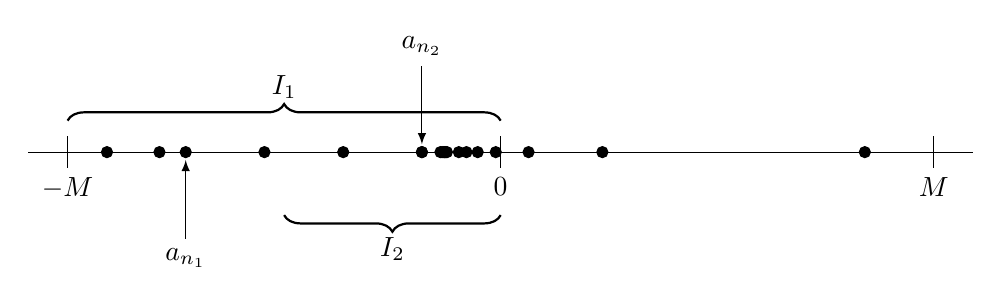
\begin{tikzpicture}[decoration={brace, amplitude=6pt}]
                  \draw (-6,0) -- (6,0) (0,0.2) -- (0,-0.2) node[below]{$0$}
                  foreach \X in {-,} {(\X5.5,0.2) -- (\X5.5,-0.2) node[below] {$\X M$}} ;
                  \draw[only marks,mark=*]
                  plot[samples at={1,...,15}] ({-1+5*(1+5*pow(-1,\x)/(2+\x))/\x},0)
                  plot[samples at={1,...,5}] ({-\x},0);
                  \draw[decorate,thick] (-5.5,0.4) -- node[above=1ex](I1){$I_1$} (0,0.4);
                  \draw[decorate,thick] (0,-0.8) -- node[below=1ex]{$I_2$} (I1|-0,-0.8);
                  \draw[latex-] (-4,-0.1) --++ (0,-1) node[below]{$a_{n_1}$};
                  \draw[latex-] (-1,0.1) --++ (0,1) node[above]{$a_{n_2}$};
              \end{tikzpicture}
          \end{center}
          \begin{proof}
              We have that $\seq{x}{n}$ implies that $(x_{n_k})_{k \in \N}$ is monotone. Further, $\seq{x}{n}$ bounded implies that $(x_{n_k})_{k \in \N}$ is bounded. So we have a montone and bounded subsequence which is thus convergent.
          \end{proof}
    \item[]
          \begin{lemma}
              Let $\seq{x}{n}$ be a bounded sequence. There is a convergent subsequence $x_{n_k}$ such that
              $$\lim_{k \to \infty} x_{n_k} = \limsup_{n \to \infty} x_n.$$
          \end{lemma}
          \begin{proof}
              We proceed by induction. Let $y = \lim_{n \to \infty} y_n$, $y_n = \sup\{x_k \ : \ k \geq n\}$ such that $y = \limsup_{n \to \infty} y_n$. \\\\
              $P(k)$: There are $n_1 < n_2 < \cdots < n_k$ and $x_{n_1}, x_{n_2}, \ldots, x_{n_k}$ such that
              $$\underbrace{y - \frac{1}{i}}_{\rightarrow y} < x_{n_i} < \underbrace{y + \frac{1}{i}}_{\rightarrow y} \ \forall 1 \leq i \leq k$$
              which implies that $x_{n_i} \rightarrow y$ as well by squeeze theorem. \\\\
              $P(1)$: There is $n_1 \in \N$ and $x_{n_1}$ such that $y - 1 < x_{n_1} < y + 1$. \\\\
              We have $y_n \rightarrow y \implies \exists N \in \N$ such that $|y_n - y| \leq \nicefrac{1}{4} \ \forall n \geq N$. Further we have $y_n = \sup\{x_n \ : \ k \geq n\} \implies \exists x_m, m \geq n$ such that $y_n - x_m \leq \nicefrac{1}{4}$ by the characterization of suprema. Then compute
              \begin{align*}
                  |y - x_n| & = |y - y_n + y_n - x_m|                      \\
                            & \leq |y - y_n| + |y_n - x_m|                 \\
                            & \leq \frac{1}{4} + \frac{1}{4} = \frac{1}{2}
              \end{align*}
              so $y - \nicefrac{1}{2} \leq x_m \leq y + \nicefrac{1}{2} \implies y - 1 < x_m < y + 1$. \\\\
              Next, assume $P(k)$ is true: There is $n_1 < n_2 < \cdots < n_k$ and $x_{n_1}, x_{n_2}, \ldots, x_{n_k}$ such that
              $$y - \frac{1}{i} < x_{n_i} < y + \frac{1}{i} \ \forall 1 \leq i \leq k.$$
              Since $y_n \rightarrow y$, $\exists N \in \N$ such that $|y - y_n| \leq \nicefrac{1}{(4(k + 1))}$, $n \geq \max\{N, n_{k + 1}\} > N_k$. Further, we have $y_n = \sup\{x_k \ : \ k \geq n\}$ which implies there exists some $m \in \N$ with $m \geq n > n_k$ such that
              $$y_n - x_m < \frac{1}{4(k + 1)}.$$
              Therefore, we have
              \begin{alignat*}{2}
                           &  & |y - y_m|           & \leq |y - y_n| + |y_n - x_m|                      \\
                           &  &                     & \leq \frac{1}{4(k + 1)} + \frac{1}{4(k + 1)}      \\
                           &  &                     & = \frac{1}{2(k + 1)} < \frac{1}{k + 1}            \\
                  \implies &  & y - \frac{1}{k + 1} & < x_m < y + \frac{1}{k + 1}, n_{k + 1} = m > n_k.
              \end{alignat*}
              Therefore, $P(k + 1)$ is true. Thus, we have shown that $P(k)$ is true for all $k \in \N$ and $x_{n_k} \rightarrow y$ by the squeeze theorem.
          \end{proof}
    \item \textbf{Remark}. Every bounded sequence $\seq{x}{n}$ has a convergent subsequence $(x_{n_k})_{k \in \N}$ such that
          $$\lim_{k \to \infty} x_{n_k} = \liminf_{n \to \infty} x_n.$$
          (Proof is the same).
    \item \textbf{Result} (forgot to mention last class). If $\seq{x}{n}$ is bounded, then every convergent subsequence $\sseq{x}{n}{k}$ satisfies
          $$\liminf_{n \to \infty} x_n \leq \lim_{k \to \infty} x_{n_k} \leq \limsup_{n \to \infty} x_n.$$
    \item \textbf{Example}. Take $x_n = (-1)^n$. We want to find the $\limsup$. \\\\
          Show that $\seq{x}{n}$ is bounded, i.e., $x_n \leq 1 \implies \limsup_{n \to \infty} \leq 1$. Then, consider the subsequence $(x_{2k}) = (1)_{k \in \N}$. Then show that $(x_{2k}) \rightarrow_{k \to \infty} 1 \implies 1 \leq \limsup_{n \to \infty} x_n$. \\\\
          Since we have shown that $\limsup_{n \to \infty} x_n \leq 1 \leq \limsup_{n \to \infty} x_n$, we know that $\limsup_{n \to \infty} x_n = 1$.
\end{itemize}

\subsection{Cauchy Sequences}

\begin{itemize}
    \item[]
          \begin{definition}[Cauchy sequences]
              A sequence $\seq{x}{n}$ is \textbf{Cauchy} if $\forall \varepsilon > 0, \exists N \in \N$ with
              $$|x_m - x_n| \leq \varepsilon \ \forall m, n \geq N.$$
          \end{definition}
    \item \textbf{Example}. Take $x_n = \nicefrac{1}{2}(x_{n - 1} + x_{n - 2}), x_0 = 0, x_1 = 1$. Then we compute
          \begin{align*}
              x_n - x_{n - 1} & = \frac{1}{2}(x_{n - 1} + x_{n - 2}) - x_{n - 1}             \\
                              & = \frac{1}{2}(x_{n - 2} - x_{n - 1})                         \\
              x_2 - x_1       & = -\frac{1}{2} \implies x_2 = -\frac{1}{2} + 1 = \frac{1}{2} \\
              x_3 - x_2       & = \frac{1}{2}(1 - \frac{1}{2}) = \left(\frac{1}{2}\right)^2.
          \end{align*}
          Then, by induction we can show that
          $$x_n - x_{n - 1} = \left(-\frac{1}{2}\right)^{n - 1}.$$
          Now take $m \geq n$ and compute
          \begin{align*}
              x_m - x_n   & = x_m - x_{m - 1} + x_{m - 1} - x_{m - 2} \pm \cdots \pm x_{n + 1} - x_n                                                              \\
              |x_m - x_n| & \leq \left(\frac{1}{2}\right)^{m - 1} + \left(\frac{1}{2}\right)^{m - 2} + \cdots + \left(\frac{1}{2}\right)^n                        \\
                          & = \left(\frac{1}{2}\right)^n\left(1 + \frac{1}{2} + \left(\frac{1}{2}\right)^2 + \cdots + \left(\frac{1}{2}\right)^{m - n - 1}\right) \\
                          & = \frac{1 - \left(\frac{1}{2}\right)^{m - 2}}{1 - \frac{1}{2}} \leq 2 \text{ (by geometric sum)}                                      \\
                          & \leq 2^{-n + 1}.
          \end{align*}
          Given $\varepsilon > 0$, if we want $2^{-n + 1} \leq \varepsilon$, compute
          \begin{align*}
              2^{-n + 1} & \leq \varepsilon      \\
              -n + 1     & \leq \ln(\varepsilon) \\
              n \geq \ln(\varepsilon) + 1.
          \end{align*}
          Therefore, take $N = \lfloor \ln(\varepsilon) \rfloor + 2$, $n \geq \ln(\varepsilon) + 1$. So, for $m, n \geq N \implies |x_m - x_n| \leq \varepsilon \implies x_n$ Cauchy. In fact, $\lim_{n \to \infty} x_n = \nicefrac{2}{3}$ (details left to reader). \\\\
          \textbf{Warning}: Checking the difference between two subsequent terms of the sequence is not enough to ensure that the sequence is Cauchy. \\\\
          For example, consider $x_n = \sum_{k = 1}^n \nicefrac{1}{k}$ (which is not Cauchy).
    \item[]
          \begin{lemma}
              A sequence $\seq{x}{n}$ is convergent if and only if $\seq{x}{n}$ is Cauchy.
          \end{lemma}
          \begin{proof}
              First, assume that $x_n \rightarrow x$. Therefore, $\forall \varepsilon > 0, \ \exists N \in \N$ such that
              $$|x_n - x| \leq \frac{\varepsilon}{2} \ \forall n \geq N.$$
              Therefore, for $\varepsilon > 0$ and $m, n \geq N$,
              $$|x - x_m| \leq \frac{\varepsilon}{2} \text{ and } |x - x_n| \leq \frac{\varepsilon}{2}.$$
              This implies that
              \begin{align*}
                  |x_m - x_n| & = |x - x_m + x - x_n|                                            \\
                              & \leq |x - x_n| + |x - x_m|                                       \\
                              & \leq \frac{\varepsilon}{2} + \frac{\varepsilon}{2} = \varepsilon \\
                              & \implies x_n \text{ Cauchy}.
              \end{align*}
              For the other direction, assume $\seq{x}{n}$ is Cauchy. First, we must prove some claims that will lead us to this proof.
              \begin{enumerate}[label=(\arabic*)]
                  \item \textbf{Claim}. If $\seq{x}{n}$ is Cauchy, then $\seq{x}{n}$ bounded.
                        \begin{proof}
                            This proof is omitted because it is almost identical to the proof as convergent implies bounded.
                        \end{proof}
                  \item \textbf{Claim}. If $\seq{x}{n}$ has a convergent subsequence $(x_{n_k})_{k \in \N}$, then $\seq{x}{n}$ is convergent (to the same limit).
                        \begin{proof}
                            To see this, assume there exists some $(x_{n_k})$ convergent subsequence and
                            \begin{enumerate}[label=(\roman*)]
                                \item We know $x_n$ is Cauchy, i,e,, $\forall \varepsilon > 0, \ \exists N_1 \in \N$ such that
                                      $$|x_m - x_n| \leq \frac{\varepsilon}{2} \ \forall m, n \geq N_1.$$
                                \item There exists an $x \in \N$ such that $\forall \varepsilon > 0, \ \exists N_2 \in \N$ such that
                                      $$|x - x_{n_k}| \leq \frac{\varepsilon}{2} \ \forall k \geq N_2.$$
                            \end{enumerate}
                            Now, we will show that the entire sequence $(x_n)$ converges to $x$. \\\\
                            For every $\varepsilon > 0$, set $N = \max{N_1, N_2}$. Then compute
                            \begin{align*}
                                |x - x_k| & \leq |x - x_{n_k}| + |x_{n_k} - x_k|                                   \\
                                          & \leq \frac{\varepsilon}{2} + \frac{\varepsilon}{2} \ \forall k \geq N.
                            \end{align*}
                        \end{proof}
              \end{enumerate}
              So, we have
              \begin{alignat*}{2}
                  (x_n) \text{ Cauchy } &  & \xRightarrow{\text{(1)}} (x_n)    & \text{ bounded }                     \\
                                        &  & \xRightarrow{\text{(B.W.)}} (x_n) & \text{ has a convergent subsequence} \\
                                        &  & \xRightarrow{\text{(2)}} (x_n)    & \text{ convergent}.
              \end{alignat*}
          \end{proof}
\end{itemize}

\subsection{Divergent Sequences to $\pm \infty$ (Unbounded Case)}

\begin{itemize}
    \item[]
          \begin{definition}[Divergence to $\pm \infty$]
              We say that a sequence $\seq{x}{n}$ is \textbf{diverging to} $+\infty$ if $\forall M \in \R, \ \exists N \in \N$ such that
              $$x_n \geq M \ \forall n \geq M.$$
              Similarly, we say that a sequence is \textbf{diverging to} $-\infty$ if $\forall M \in \R, \ \exists N \in \N$ such that
              $$x_n \leq M \ \forall n \geq N.$$
          \end{definition}
    \item[]
          \begin{lemma}
              If $\seq{x}{n}$ is converging to $\pm \infty$, then every subsequence is convering to $\pm \infty$ (respectively).
          \end{lemma}
\end{itemize}

\section{Continuous Functions}

\begin{itemize}
    \item[]
          \begin{definition}[Functional limits]
              Let $a < b$, $x_0 \in (a, b), f:(a, b) \setminus \{x_0\} \mapsto \R$. We say that $f$ \textbf{has a limit} $l$ at $x_0$ if $\forall \varepsilon > 0 \ \exists \delta > 0$ such that, for $x \in (a, b)$
              $$0 < |x - x_0| \leq \delta \implies |f(x) - l| \leq \varepsilon.$$
              If $f$ has a limit $l$, we write
              $$\lim_{x \to x_0} f(x) = l.$$
          \end{definition}
          \begin{center}
              \begin{tikzpicture}]
                  \begin{axis}[ axis lines=middle, xlabel = $x$, ylabel = {$y$}, ymax=20, ymin=0,
                          extra x ticks={3,5,7},
                          extra y ticks={4.5,6.5,8.5}, xtick={\empty}, ytick={\empty},
                          extra y tick labels={$L-\varepsilon$,$L$,$L+\varepsilon$},
                          extra x tick labels={$a-\delta$,$a$,$a+\delta$},
                          extra tick style={grid=major}, grid style={dashed},
                          axis y line=left, axis x line=bottom, ]
                      \addplot[domain=-4:8, color=red]{0.5*(x-2)^2+2} node[pos=.1,right] {$f(x)$};
                      \addplot coordinates {(5,6.5)};
                      \draw[dashed,blue] (axis cs:5,0)--(axis cs:5,20);
                      \draw[dashed,blue] (axis cs:-4,6.5)--(axis cs:8,6.5);
                  \end{axis}
              \end{tikzpicture}
          \end{center}
    \item[]
          \begin{proposition}
              Let $x_0 \in (a, b), f: (a, b) \setminus \{x_0\} \mapsto \R$. If $f$ has a limit at $x_0$, then the limit must be unique.
          \end{proposition}
          \begin{proof}
              For the sake of contradiction, assume that $l_1, l_2$ are two limits of $f$ at $x_0$ and further assume that $l_1 < l_2$. Take $\varepsilon = (l_2 - l_1) / 4$. Then we have
              \begin{itemize}[label=\smallblacksquare]
                  \item $l_1$ a limit means $\exists \delta_1 > 0$ such that
                        $$0 < |x - x_0| \leq \delta_1 \implies |f(x) - l_1| \leq \varepsilon.$$
                  \item $l_2$ a limit means $\exists \delta_2 > 0$ such that
                        $$0 < |x - x_0| \leq \delta_2 \implies |f(x) - l_2| \leq \varepsilon.$$
              \end{itemize}
              Then, compute for $0 < |x - x_0| \leq \min\{\delta_1, \delta_2\}$
              \begin{align*}
                  l_2 - l_1 & \leq |l_2 - f(x)| + |l_1 - f(x)|              \\
                            & \leq \varepsilon + \varepsilon = 2\varepsilon \\
                            & = \frac{l_2 - l_1}{2} < l_2 - l_1.
              \end{align*}
              Of course, this is a contradiction so $l_1 = l_2$.
          \end{proof}
    \item \textbf{Example}. Take $f(x) = x^2$. We wish to show that $\lim_{x \to 2} f(x) = 4$. To show, we have $\forall \varepsilon > 0 \ \exists \delta > 0$ such that
          $$0 < |x - 2| \leq \delta \implies |x^2 - 4| \leq \varepsilon.$$
          Then, compute
          \begin{align*}
              |x^2 - 4|    & = \underbrace{|x - 2|}_{\leq \delta}|x + 2| \\
                           & \leq \delta(|x| + 2)                        \\
                           & \leq \delta(4 + \delta)                     \\
              \implies |x| & \leq 2 + \delta
          \end{align*}
          (since $|x| = |x - 2 + 2| \leq |x - 2| + 2$). Now we want $\delta(4 + \delta) \leq \varepsilon$. Further, restrict $\delta \leq 1 \implies \delta^2 \leq \delta$ and $\delta(4 + \delta) \leq 5\delta$. We must now show that $5\delta \leq \varepsilon$. \\\\
          So, $\forall \varepsilon > 0$, set $\delta = \min\{1, \nicefrac{\varepsilon}{5}\}$. Then
          $$0 < |x - 2| \leq \delta \implies |x^2 - 4| \leq 5\delta \leq \varepsilon.$$
          So indeed $\lim_{x \to 2} f(x) = 4$.
    \item \textbf{Example}. Take $f(x) = (x - 1)/(x - 1), x \neq 1$. This function is not defined at $x = 1$, so take $f: (-2, 2) \setminus \{1\} \mapsto \R$. However, we claim still that $\lim_{x \to \infty} f(x) = 1$. We show $\forall \varepsilon > 0$, set $\delta = 1$. Then we have
          $$0 < |x - 1| \leq \delta \implies |f(x) - 1| = |1 - 1| = 0 \leq \varepsilon.$$
\end{itemize}

\subsection{Sequential Limits}

\begin{itemize}
    \item[]
          \begin{proposition}
              Let $x_0 \in (a, b), f: (a, b) \setminus \{x_0\} \mapsto \R$. Then $f$ has the limit $l$ at $x_0$ if and only if for every sequence $\seq{z}{n}$, $z_n \in (a, b) \setminus \{x_0\}$ with $z_n \rightarrow x_0$, then the sequence $(f(z_n))_{n \in \N}$ has
              $$f(z_n) \rightarrow l.$$
              \label{prop:seq_lim}
          \end{proposition}
          \begin{proof}
              First, suppose $\lim_{x \to x_0} f(x) = l$ and $\seq{z}{n}, z_n \in (a, b) \setminus \{x_0\}$ with $z_n \rightarrow x_0$. Then, we know the following
              \begin{enumerate}[label=(\arabic*)]
                  \item $\lim_{x \to x_0} f(x) = l \implies \forall \varepsilon > 0 \ \exists \delta > 0$ such that $0 < |x - x_0| \leq \delta \implies |f(x) - l| \leq \varepsilon$ and
                  \item $z_n \rightarrow x_0 \implies \forall \widetilde{\varepsilon} \ \exists \widetilde{N} \in \N$ such that $|z_n - x_0| \leq \widetilde{\varepsilon} \ \forall n \geq \widetilde{N}$.
              \end{enumerate}
              Then, let $\varepsilon > 0$ be given. Set $\widetilde{\varepsilon} = \delta$ so that $n \geq N \implies 0 < |z_n - x_0| \leq \delta$ and then together with (1) this implies $|f(z_n) - l| \leq \varepsilon$. Of course, this means $\lim_{n \to \infty} f(z_n) = l$ by definition. \\\\
              For the other direction, assume by contradiction that $\lim_{x \to x_0} f(x) \neq l$. By definition, this implies that $\exists \varepsilon_0 \geq 0$ such that $\forall \delta > 0$ and $0 < |x - x_0| \leq \delta \implies |f(x) - l| > \varepsilon_0$. Now, let $n \in \N$ and $z_n \in (x_0 - \nicefrac{1}{n}, x_0 + \nicefrac{1}{n}) \setminus \{x_0\}$. By the Squeeze Theorem (Theorem~\ref{thm:squeeze})
              $$x_0 - \frac{1}{n} \leq z_n \leq x_0 + \frac{1}{n} \implies z_n \rightarrow x_0.$$
              By assumption, $\lim_{n \to \infty} f(z_n) = l$, i.e., $\forall \varepsilon > 0 \ \exists n \in \N$ such that $\forall n \geq N$, $|f(z_n) - l| \leq \varepsilon$. Taking $\delta = \nicefrac{1}{n}$, we obtain a contradiction. Therefore, our contradiction assumption must be false and $\lim_{x \to x_0} f(x) = l$.
          \end{proof}
    \item \textbf{Example}. Take $f(x) = \nicefrac{x}{|x|}, x \neq 0$. How do we show that this does not have a limit at $x = 0$? We could use the epsilon-delta proof technique, but this could be long and tedious. Instead, consider
          \begin{align*}
              \text{Let } z_n             & = -\frac{1}{n} \rightarrow 0 \\
              f(z_n)                      & = -1 \rightarrow -1          \\
              \text{Let } \widetilde{z_n} & = \frac{1}{n} \rightarrow 0  \\
              f(\widetilde{z_n})          & = 1 \rightarrow 1
          \end{align*}
          $\implies f(x)$ does not have a limit at $x_0$.
    \item \textbf{Corollary}. Let $x_0 \in (a, b) \setminus \{x_0\}$, $f: (a, b) \mapsto \R$. Assume that every sequence $\seq{z}{n}$, $z_n \in (a, b) \setminus \{x_0\}$, $z_n \rightarrow x_0$, one has $(f(z_n))_{n \in \N}$ is convergent. Then $f$ has a limit at $x_0$.
          \begin{proof}
              We will show that for $\seq{v}{n}$, $\seq{w}{n}$ two sequences with $v_n, w_n \in (a, b) \setminus \{z_0\}$ and $v_n \rightarrow x_0, w_n \rightarrow x_0$, one has $\lim_{n \to \infty} f(v_n) = \lim_{n \to \infty} f(w_n)$. \\\\
              For the sake of contradiction, assume $l_1 = \lim{n \to \infty} f(v_n) \neq \lim_{n \to \infty} f(w_n) = l_2$. Set
              \[ y_n =
                  \begin{cases}
                      v_n & n \text{ even} \\
                      w_n & n \text{ odd}.
                  \end{cases}
              \]
              Then we have (1) $y_n \in (a, b) \setminus \{x_0\}$ and (2) $y_n \rightarrow x_0$ together imply $(f(y_n))_{n \in \N}$ convergent. However,
              \[
                  f(y_n) =
                  \begin{cases}
                      f(v_n) & n \text{ even} \\
                      f(w_n) & n \text{ odd}
                  \end{cases}
              \]
              cannot be convergent since $f(y_{2n}) \rightarrow l_2$ and $f(y_{2n + 1}) \rightarrow l_2$ which contradicts our assumption that $l_1 \neq l_2$. Therefore, our assumption must be false and $l_1 = l_2$. Combining this with our previous result (Proposition~\ref{prop:seq_lim}) we get that $\lim_{x \to x_0} f(x) = l_1 = l_2$.
          \end{proof}
          \begin{lemma}[Cauchy Criteria for Functions]
              Let $x_0 \in (a, b) \setminus \{x_0\}, f: (a, b) \setminus \{x_0\} \mapsto \R$. Then $f$ has a limit at $x_0$ if and only if for every $\varepsilon > 0$, there exists $\delta > 0$ such that for every $x_1, x_2$ satisfying
              $$0 < |x_1 - x_0| \leq \delta \qquad 0 < |x_2 - x_1| \leq \delta,$$
              one has
              $$|f(x_1) - f(x_2)| \leq \varepsilon.$$
              \label{lemma:cauchy_crit}
          \end{lemma}
          \begin{proof}
              First, assume that $\lim_{x \to x_0} f(x) = l$. This implies that $\forall \varepsilon > 0 \ \exists \delta > 0$ such that $|0 < |x - x_0| \leq \delta \implies |f(x) - l| \leq \nicefrac{\varepsilon}{2}$. Let $\varepsilon > 0$ be given, then there exists some $\delta > 0$ such that $0 < |x_1 - x_2| \leq \delta$ and $0 < |x_2 - x_1| \leq \delta \implies |f(x_i) - l| \leq \nicefrac{\delta}{2}$ for $i = 1, 2$. Therefore,
              \begin{align*}
                  |f(x_1) - f(x_2)| & \leq |f(x_1) - l| + |f(x_2) - l|                                  \\
                                    & \leq \frac{\varepsilon}{2} + \frac{\varepsilon}{2} = \varepsilon.
              \end{align*}
              For the other direction, we will show that for every sequence $\seq{z}{n}$, $z_n \in (a, b) \setminus \{x_0\}$, $(f(z_n))_{n \in \N}$ is convergent (Corollary implies $f$ has a limit at $x_0$). Recall the fact that $(f(z_n))_{n \in \N}$ convergent $\iff (f(z_n))_{n \in \N}$ Cauchy. Thus, we only need to show that $\forall \varepsilon > 0 \ \exists n \in \N$ such that $\forall m, n \geq N$, $|f(z_n) - f(z_m)| \leq \varepsilon$. Since $z_n \rightarrow x_0$ by assumption, we also know that for every $\delta > 0, \ \exists N \in \N$ such that $\forall n \geq N$, $0 < |z_n - x_0| \leq \delta$. \\\\
              Putting everything together, we get that $\forall \varepsilon > 0, \ \exists N \in \N$ and $0 < |x_0 - z_n| \leq \delta \ \forall n \geq N$ which in turn implies that $|f(z_n) - f(z_m)| \leq \varepsilon \ \forall m, n \geq N$. So, we know that $(f(z_n))_{n \in \N}$ is Cauchy. Therefore, $(f(z_n))_{n \in \N}$ is convergent.
          \end{proof}
\end{itemize}

\subsection{Algebraic Manipulation of Continuous Limits}

\begin{itemize}
    \item The theme of this subsection is: ``everything we know about sequences holds for limits of continuous functions."
    \item[]
          \begin{lemma}
              Let $f, g: (a, b) \setminus\{x_0\} \mapsto \R$ with $\lim_{x \to x_0} f(x) = l_1$ and $\lim_{x \to x_0} g(x) = l_2$. Then
              \begin{enumerate}[label=(\arabic*)]
                  \item $f + g$ has a limit at $x_0$ and $\lim_{x \to x_0} (f + g) = l_1 + l_2$.
                  \item For $\lambda \in \R$, $\lambda \cdot f$ has a limit at $x_0$ and $\lim_{x \to x_0} (\lambda \cdot f) = \lambda \cdot l_1$.
                  \item $f \cdot g$ has a limit at $x_0$ and $\lim_{x \to x_0} (f \cdot g) = l_1 \cdot l_2$.
                  \item Assume $f(x) \neq 0, x \in (a, b) \setminus\{x_0\}$ and $l_1 \neq 0$. Then $\nicefrac{g}{f}$ has a limit at $x_0$ and $\lim_{x \to x_0} (\nicefrac{g}{f}) = \nicefrac{l_2}{l_1}$.
              \end{enumerate}
          \end{lemma}
          \begin{proof}
              \begin{enumerate}[label=(\arabic*)]
                  \item Let $\seq{z}{n}$, $z_n \in (a, b) \setminus\{x_0\}$, $z_n \rightarrow x_0$. We know that
                        \begin{align*}
                            \lim_{x \to x_0} f(x) = l_1 & \implies f(z_n) \rightarrow l_1, \\
                            \lim_{x \to x_0} g(x) = l_2 & \implies g(z_n) \rightarrow l_2.
                        \end{align*}
                        Then, using the properties of sequences,
                        $$\lim_{n \to \infty} (f(z_n) + g(z_n)) = l_1 + l_2$$
                        which implies that $\lim_{x \to x_0} (f + g)(x) = l_1 + l_2$.
              \end{enumerate}
          \end{proof}
\end{itemize}

\subsection{Comparison Results}

\begin{itemize}
    \item[]
          \begin{lemma}
              Let $f, g: (a, b) \setminus\{x_0\} \mapsto \R$. Assume further that
              \begin{enumerate}[label=(\arabic*)]
                  \item $\lim_{x \to x_0} f(x) = l_1$ and $\lim_{x \to x_0} g(x) = l_2$ and
                  \item $\exists \alpha > 0$ such that $0 < |x - x_0| \leq \alpha \implies f(x) \geq g(x)$.
              \end{enumerate}
              Then $l_1 \geq l_2$.
              \label{lemma:three_four_one}
          \end{lemma}
          \begin{proof}
              Let $\seq{z}{n}$, $z_n \in (a, b) \setminus\{x_0\}, z_n \rightarrow x_0$. This tells us that $\exists N \in \N$ such that $\forall n \geq N, 0 < |z_n - x_0| \leq \alpha \overset{(2)}{\implies} f(z_n) \geq g(z_n) \ \forall n \geq N$. \\\\
              Then, using the properties of sequences, we get that
              $$l_1 = \lim_{n \to \infty} f(z_n) \geq \lim_{n \to \infty} g(z_n) = l_2.$$
          \end{proof}
    \item[]
          \begin{lemma}
              Let $f: (a, b) \setminus \{x_0\} \mapsto \R$ such that $\lim_{x \to x_0} f(x) = l$. Then $\lim_{x \to x_0} |f(x)| = |l|$.
          \end{lemma}
          \begin{proof}
              By the reverse triangle inequality, we have $0 \leq ||f| - |l|| \leq |f - l|$. Then, let
              \[
                  f(x) =
                  \begin{cases}
                      1  & x \in \Q               \\
                      -1 & x \in \R \setminus \Q.
                  \end{cases}
              \]
              Then $|f(x)| = 1 \implies \lim_{x \to 0} |f|(x) = 1$. But $\delta > 0$ in $(0, \delta)$ there is always
              \begin{align*}
                  x_1 & \in \Q \cap (0, \delta)               \\
                  x_2 & \in \R \setminus \Q \cap (0, \delta).
              \end{align*}
              We know further that $|f(x_1) - f(x_2)| = 2$ which implies that $f$ does not have a limit at 0 since $x_1$ and $x_2$ do not satisfy the criteria of a Cauchy sequence (Lemma ~\ref{lemma:cauchy_crit}).
          \end{proof}
    \item[]
          \begin{theorem}[Squeeze Theorem]
              Let $f, g, h: (a, b) \setminus \{x_0\} \mapsto \R$. Further, assume
              \begin{enumerate}[label=(\arabic*)]
                  \item $\lim_{x \to x_0} f(x) = l = \lim_{x \to x_0} g(x)$ and
                  \item $\exists \alpha > 0$ such that $0 < |x - x_0| \leq \alpha$.
              \end{enumerate}
              Then $\lim_{x \to x_0} h(x) = l$.
          \end{theorem}
          \begin{proof}
              Let $\seq{z}{n}$, $z_n \in (a, b) \setminus \{x_0\}, z_n \rightarrow x_0$. This means $\exists N \in \N$ such that $\forall n \geq N$, $0 < |z_n - x_0| \leq \alpha$. By (2) of Lemma ~\ref{lemma:three_four_one}, we have that $$f(z_n) \leq h(z_n) \leq g(z_n) \ \forall n \geq N.$$
              Therefore, we have $\lim_{n \to \infty} h(z_n) = l$ and because $\seq{z}{n}$ is arbitrary, $\lim_{x \to x_0} h(x) = l$.
          \end{proof}
    \item \textbf{Example}. Take $f: (-\nicefrac{\pi}{2}, \nicefrac{\pi}{2}) \setminus \{0\} \mapsto \R$ defined by $f(x) = \nicefrac{\sin x}{x}, x > 0$. How can we show that $\lim_{x \to 0} f(x) = 1$? We could show this rigorously with the definition of limits, however this would be tedious. Instead, consider that we know $\sin x \leq x$. In particular,
          \begin{align*}
              |1 - \cos x| & = 2\left|\sin^2 \frac{x}{2}\right| \leq \frac{x^2}{2}.
          \end{align*}
          This implies that $\lim_{x \to 0} \cos x = 1$. On the other hand,
          $$\frac{\sin x}{2} \leq \pi \cdot \frac{x}{2\pi} \leq \frac{\tan x}{2}$$
          and for $x \neq 0$, we obtain
          $$1 \leq \frac{x}{\sin x} \leq 1.$$
          Since $\cos x \underset{x \to 0}{\longrightarrow} 1$ and $1 \underset{1 \to 0}{\longrightarrow} 1$, we have by the squeeze theorem for functions that $\lim_{x \to 0} \nicefrac{\sin x}{x} = 1$.
\end{itemize}

\subsection{Composition of Functions}

\begin{itemize}
    \item[]
          \begin{lemma}[Composition of Functions]
              Let $f: (a, b) \setminus \{x_0\} \mapsto (c, d)$ such that $\lim_{x \to x_0} f(x) = y_0$. Let $g: (c, d) \setminus \{y_0\} \mapsto \R$ and assume that $\lim_{y \to y_0} g(y) = l$. Then $g \circ f$ has a limit at $x_0$ and $\lim_{x \to x_0} (g \circ f)(x) = l$. \\\\
              Note: we must assume $\exists \alpha > 0$ such that $0 < |x - x_0| \leq \alpha \implies f(x) = y_0$).
          \end{lemma}
          \begin{proof}
              We know two things by assumption:
              \begin{enumerate}[label=(\arabic*)]
                  \item $\lim_{x \to x_0} f(x) = y_0$ means
                        $$\forall \varepsilon_1 > 0 \ \exists \delta_1 > 0 \text{ such that } 0 < |x - x_0| \leq \delta_1 \implies |f(x) - y_0| \leq \varepsilon_1.$$
                  \item $\lim_{y \to y_0} g(y) = l$ means
                        $$\forall \varepsilon_2 > 0 \ \exists \delta_2 > 0 \text{ such that } 0 < |y - y_0| \leq \delta_2 \implies |g(y) - l| \leq \varepsilon_2.$$
                        Here, we further assume that $\exists \alpha > 0$ such that $0 < |x - x_0| \leq \alpha \implies f(x) \neq y_0$. Altogether this implies that
                        $$0 \leq |x - x_0| \leq \min\{\delta_1, \alpha\} \implies 0 < |f(x) - y_0| \leq \varepsilon_1.$$
              \end{enumerate}
              So we want to show that $\forall \varepsilon > 0 \ \exists \delta > 0$ such that
              $$0 < |x - x_0| \leq \delta \implies |g(f(x)) - l| \leq \varepsilon.$$
              Let $\varepsilon > 0$ be given. Set $\varepsilon_2 = \varepsilon \implies \exists \delta_2$, set $\varepsilon_1 = \delta_2 \implies \delta_1$ and then set $\delta = \min\{\delta_1, \alpha\}$. Thus,
              \begin{align*}
                  0 < |x - x_0| \leq \delta & \implies 0 < |\underbrace{f(x)}_{= y} - y_0| \leq \varepsilon_1 = \delta_2 \\
                                            & \implies |g(f(x)) - l| \leq \varepsilon.
              \end{align*}
          \end{proof}
\end{itemize}

\subsection{Infinite Limits}

\begin{itemize}
    \item[]
          \begin{definition}[Infinite functional limits]
              We say that $f: (a, b) \setminus \{x_0\} \mapsto \R$ \textbf{tends to} $+\infty$ when $x$ tends to $x_0$ if $\forall M \in \R \ \exists \delta > 0$ such that
              $$0 < |x - x_0| \leq \delta \implies f(x) \geq M.$$
              We write $\lim_{x \to x_0} f(x) = +\infty$. \\\\
              Similarly, we say that $f$ \textbf{tends to } $-\infty$ when $x$ tends to $x_0$ if $\forall M \in \R \ \exists \delta > 0$ such that
              $$0 < |x - x_0| \leq \delta \implies f(x) \leq M.$$
              We write $\lim_{x \to x_0} f(x) = -\infty$.
          \end{definition}
    \item[]
          \begin{definition}[Infinite functional limits]
              We say that $f: (a, +\infty) \mapsto \R$ has a limit $l$ when $x$ tends to $+\infty$ if $\forall \varepsilon > 0 \ \exists D \in \R$ such that
              $$x \geq D \implies |f(x) - l| \leq \varepsilon.$$
              We write $\lim_{x \to +\infty} f(x) = l$. \\\\
              Similarly, we say that $f: (-\infty, b) \mapsto \R$ has a limit $l$ when $x$ tends to $-\infty$ if $\forall \varepsilon > 0 \ \exists D \in \R$ such that
              $$x \leq D \implies |f(x) - l| \leq \varepsilon.$$
              We write $\lim_{x \to -\infty} f(x) = l$.
          \end{definition}
    \item[]
          \begin{definition}[Combined infinite functional limits]
              We say that $f: (a, +\infty) \mapsto \R$ tends to $+\infty$ when $x \rightarrow +\infty$ if $\forall M \in \R \ \exists D \in \R$ such that
              $$x \geq D \implies f(x) \geq M.$$
              We write $\lim_{x \to +\infty} f(x) = +\infty$. \\\\
              Similarly, we say that $f: (-\infty, b) \mapsto \R$ tends to $-\infty$ when $x \rightarrow -\infty$ if $\forall M \in \R \ \exists D \in \R$ such that
              $$x \leq D \implies f(x) \leq M.$$
              We write $\lim_{x \to -\infty} f(x) = -\infty$.
          \end{definition}
\end{itemize}

\subsection{Continuity}

\begin{itemize}
    \item[]
          \begin{definition}[Functional continuity]
              We say that $f: (a, b) \mapsto \R$ is \textbf{continuous} at $x_0 \in (a, b)$ if
              $$\lim_{x \to x_0} f(x) = f(x_0).$$
              This is equivalent to:
              \begin{enumerate}[label=(\roman*)]
                  \item $\forall \varepsilon > 0 \ \exists \delta(\varepsilon, x_0) > 0$ such that $|x - x_0| \leq \delta \implies |f(x) - f(x_0)| \leq \varepsilon$.
                        \begin{proof}
                            Left as an exercise.
                        \end{proof}
                  \item $\forall \varepsilon > 0 \ \exists \delta(\varepsilon, x_0) > 0$ such that $|x_1 - x_0| \leq \delta$ and $|x_2 - x_0| \leq \delta \implies |f(x_1) - f(x_2)| \leq \varepsilon$.
                        \begin{proof}
                            Left as an exercise.
                        \end{proof}
              \end{enumerate}
          \end{definition}
    \item[]
          \begin{lemma}
              Let $x_0 \in (a, b)$ and $f: (a, b) \mapsto \R$. Then $f$ is continuous at $x_0$ if and only if for every sequence $\seq{z}{n}$, $z_n \in (a, b)$, $z_n \rightarrow x_0$,
              $$f(z_n) \rightarrow f(x_0).$$
          \end{lemma}\
          \begin{proof}
              First, assume that $f$ is continuous at $x_0$. In other words, $\lim_{x \to x_0} f(x) = f(x_0)$. Let the sequence $\seq{z}{n}$, $z_n \in (a, b)$, $z_n \rightarrow x_0$. Let $\varepsilon > 0$ be given. Then $\exists N \in \N$ such that $\forall n \geq N (z_n \neq x_0)^*$,
              \begin{align*}
                           & |f(z_n) - f(x_0)| \leq \varepsilon \\
                  \implies & f(z_n) \longrightarrow f(x_0).
              \end{align*}
              For the other direction, assume that every sequence $\seq{z}{n}$, $z_n \in (a, b)$, $z_n \rightarrow x_0 \implies f(z_n) \rightarrow f(x_0)$. In particular, consider the sequences $\seq{z}{n}$, $z_n \in (a, b) \setminus \{x_0\}$, $z_n \rightarrow x_0 \implies f(z_n) \rightarrow f(x_0) \implies \lim_{x \to x_0} f(x) = \lim_{n \to \infty} f(z_n) = f(x_0)$.
          \end{proof}
    \item \textbf{Example}. Take $f: (0, +\infty) \mapsto \R$ be defined by $f(x) = \sqrt{x}$. We claim that $f$ is continuous at every $x_0 \in (0, +\infty)$. Set $x \in (0, +\infty$ and compute
          \begin{align*}
              |f(x) - f(x_0)| = |\sqrt{x} - \sqrt{x_0}| = \frac{|x - x_0|}{\underbrace{\sqrt{x}}_{> 0} + \sqrt{x_0}} \leq \frac{|x - x_0|}{\sqrt{x_0}}.
          \end{align*}
          Now, $\forall \varepsilon > 0$ set $\delta = \varepsilon \cdot \sqrt{x_0}$, then we have
          $$|x - x_0| \leq \delta \implies |f(x) - f(x_0)| \leq \frac{\delta}{\sqrt{x_0}} \leq \varepsilon$$
          $\implies \sqrt{x}$ is continuous at $x_0$.
    \item[]
          \begin{proposition}
              Let $f, g: (a, b) \mapsto \R$ continuous at $x_0 \in (a, b)$. Then
              \begin{enumerate}[label=(\roman*)]
                  \item $f + g$ is continuous at $x_0$
                  \item For $\lambda \in \R$, $\lambda \cdot f$ is continuous at $x_0$
                  \item $f \cdot g$ is continuous at $x_0$
                  \item $f \neq 0$ on $(a, b)$, $\nicefrac{g}{f}$ is continuous at $x_0$
                  \item $f: (a, b) \mapsto (c, d), g: (c, d) \mapsto \R$, $f$ is continuous at $x_0 \in (a, b)$ and $g$ is continuous at $f(x_0) \in (c, d)$, then $g \circ f$ is continuous at $x_0$.
              \end{enumerate}
          \end{proposition}
          \begin{proof}
              Left as an exercise.
          \end{proof}
    \item \textbf{Example}. Let $f: (0, +\infty) \mapsto \R$. We claim $f(x) = \sqrt{x}$ is continuous at every $x_0 \in (0, +\infty)$. \\\\
          Consider $f: \R \mapsto \R$ defined by
          \[
              f(x) =
              \begin{cases}
                  1 & x \in \Q              \\
                  0 & x \in \R \setminus \Q
              \end{cases}
          \]
          which is discontinuous everywhere. Then let $x_0 \in \R, n \in \N$. We know that there exists $a_n, b_n \in (x_0 - \nicefrac{1}{n}, x_0 + \nicefrac{1}{n})$ such that $a_n \in \Q, b_n \in \R \setminus \Q$ such that $a_n, b_n \underset{n \rightarrow \infty}{\longrightarrow} x_0$. Then we have
          \begin{align*}
              f(a_n) & = 1 \rightarrow 1 \\
              f(b_n) & = 0 \rightarrow 0
          \end{align*}
          $\implies f$ discontinuous at $x_0$.
    \item[]
          \begin{definition}[Continuity on an interval]
              We say $f: (a, b) \mapsto \R$ is \textbf{continuous on $(a, b)$} if it is continuous at \textit{every} $x_0 \in (a, b)$. \\\\
              We write $f \in C^0 \big((a, b)\big)$.
          \end{definition}
    \item[]
          \begin{definition}[Left/right limits]
              Let $f: (a, b) \setminus \{x_0\} \mapsto \R$. We say that $f$ has a \textbf{left-sided limit} $l \in \R$ at $x_0$ if $\forall \varepsilon > 0 \ \exists \delta(x_0, \varepsilon) > 0$ such that
              $$\underbrace{0 < |x - x_0| \leq \delta}_{x - \delta \leq x \leq x_0} \implies |f(x) - l| \leq \varepsilon.$$
              We write $\lim_{x \to x_0^-} f(x) = x_0$. \\\\
              Similarly, we say that $f$ has a \textbf{right-sided limit} $l \in \R$ at $x_0$ if $\forall \varepsilon > 0 \ \exists \delta(x_0, \varepsilon) > 0$ such that
              $$\underbrace{0 < |x - x_0| \leq \delta}_{x_0 \leq x \leq x_0 + \delta} \implies |f(x) - l| \leq \varepsilon.$$
              We write $\lim_{x \to x_0^+} f(x) = x_0$.
          \end{definition}
    \item[]
          \begin{definition}[Left/right continuous]
              We say that $f: (a, b) \mapsto \R$ is \textbf{left-continuous} at $x_0 \in (a, b]$ if $\lim_{x \to x_0^-} f(x) = f(x_0) \iff \forall \varepsilon > 0 \ \exists \delta > 0$ such that
              $$x_0 - \delta \leq x \leq x_0 \implies |f(x) - l| \leq \varepsilon.$$
              Similarly, we say that $f: (a, b) \mapsto \R$ is \textbf{right-continuous} at $x_0 \in [a, b)$ if $\lim_{x \to x_0^+} f(x) = f(x_0) \iff \forall \varepsilon > 0 \ \exists \delta > 0$ such that
              $$x_0 \leq x \leq x_0 + \delta \implies |f(x) - l| \leq \varepsilon.$$
          \end{definition}
    \item \textbf{Example}. Let $f(x) = \sqrt{x}$. Is $f(x)$ is right-continuous at 0? i.e., $\lim_{x \to x_0^+} f(x) \overset{?}{=} 0$. We note that $f(x)$ is continuous on $(0, 1)$ but does not have a right limit at 0.
    \item[]
          \begin{lemma}
              Let $f: (a, b) \mapsto \R, x_0 \in (a, b)$. Then $f$ is continuous at $x_0$ if and only if
              $$\lim_{x \to x_0^-} f(x) = \lim_{x \to x_0^+} f(x) = f(x_0).$$
          \end{lemma}
          \begin{proof}
              Left as an exercise.
          \end{proof}
    \item[]
          \begin{definition}[Continuity on a closed interval]
              We say $f: [a, b] \mapsto \R$ is \textbf{continuous on a closed interval} if it is continuous on $(a, b)$ and $\lim_{x \to x_0^+} f(x) = f(a), \lim_{x \to x_0^-} f(x) = f(b)$. \\\\
              We write $f \in C^0\big([a, b]\big)$.
          \end{definition}
    \item[]
          \begin{theorem}[Intermediate Value Theorem]
              Let $f: (a, b) \mapsto \R$ be a continuous function such that $f(a) < f(b)$. Then for every $y_0 \in \R$ such that $f(a) < y_0 < f(b)$, there exists $x_0 \in (a, b)$ such that $f(x_0) = y_0$ (symmetrical for $f(b) < f(a)$). \\\\
              \danger \textbf{Caution}: $y_0$ may not be unique.
              \label{theorem:ivt}
          \end{theorem}
          \begin{proof}
              Let $X = \set{x \in [a, b]}{f(x) < y_0} \subset [a, b]$. We know that $X \neq \emptyset$ since $a \in X$ by definition. Further, since $X$ is a subset of a bounded set, we know that $X$ is bounded. Therefore, we know that $s = \sup(X)$ exists. \\\\
              Now, we want to show
              \begin{enumerate}[label=(\roman*)]
                  \item $a < s < b$ and
                  \item $f(x) = y_0$.
              \end{enumerate}
              If we can show these two things then we get that $x_0 = s$.
              \begin{enumerate}[label=(\roman*)]
                  \item We want to show that $a < s$. Recall that $f$ is right-continuous at a means that $\forall \varepsilon > 0 \ \exists \delta > 0$ such that
                        $$a \leq x \leq a + \delta \implies |f(x) - f(a)| \leq \varepsilon.$$
                        In particular, for $e = (y_0 - f(a)) / 2$, we obtain
                        \begin{align*}
                            a \leq x \leq a + \delta & \implies |f(x) - f(a)| \leq \varepsilon = \frac{y_0 - f(a)}{2}     \\
                                                     & \implies f(x) \leq f(a) + \varepsilon = \frac{f(a) + y_0}{2} < y_0
                        \end{align*}
                        by construction. Now for the sake of contradiction, assume that $\sup(X) = s = a$. Then take $z = \nicefrac{(a + \delta)}{2}$ and $f(z) < y_0$ by construction which further implies that $z \in X$. However, $z > a = s$ which contradicts the initial assumption that $s = \sup(X)$. Therefore, our contradiction assumption must be false and $a < s$. \\\\
                        Next, we must show that $s < b$. Recall that since $f$ is left-continuous at $b$, we have $\forall \varepsilon > 0 \ \exists \delta > 0$ such that
                        $$b - \delta \leq x \leq b \implies |f(x) - f(b)| \leq \varepsilon \implies f(x) \geq f(b) - \varepsilon.$$
                        Therefore, take $\varepsilon = f(b) - y_0 \implies f(x) \geq y_0$ by construction. For the sake of contradiction, assume that $\sup(X) = s = b$. Then we have that $b - \delta \leq x \leq b \implies x \not\in X$. So take $z = b - \nicefrac{\delta}{2}$ which means that $z \geq x \ \forall x \in X$. However, this contradicts the initial assumption that $s$ is the \textit{smallest} upper bound of $X$. Therefore our contradiction assumption must be false and $s < b$.
                  \item We want to show that $f(s) = y_0$. First, we will show that $f(s) \geq y_0$. Let $\seq{z}{n}, z_n \in (s, s + \nicefrac{1}{n}), z_n \rightarrow s$. Then we surely have that $z_n > s, z_n \not\in X$ which implies that (by the definition of $X$) $f(z_n) \geq y_0$. Note that by comparison theorems, we have that $\lim_{n \to \infty} f(z_n) \geq y_0$ (since $f(z_n) \geq y_0 \ \forall n \in \N$). Also, since $f$ is continuous on the interval, we have
                        $$y_0 \leq \lim_{n \to \infty} f(z_n) = f\big(\lim_{n \to \infty} z(n)\big) = f(s) \implies f(s) \geq y_0.$$
                        Next, we will show that $f(s) \leq y_0$. Recall the property of supremum: $\exists z_n \in X$ such that $z_n \rightarrow s$. Then we know that $f(z_n) < y_0$ since $z_n \in X$. Similarly to before, we have
                        \begin{align*}
                            y_0 \geq \lim_{n \to \infty} f(z_n) = f\left(\lim_{n \to \infty} f(z_n)\right) = f(s) \implies f(s) \leq y_0.
                        \end{align*}
              \end{enumerate}
              Together, (i) and (ii) imply that $f(s) = y_0$.
          \end{proof}
    \item \danger \textbf{Warning}: If $f: [a, b] \mapsto \R$ such that $f(a) < f(b)$ and $\forall y_0 \in \R$ with $f(a) < y_0 < f(b) \implies \exists x_0 \in (a, b)$ with $f(x_0) = y_0$
          $$\centernot\implies f \text{ is continuous on } [a, b]!$$
    \item[]
          \begin{definition}[Monotone functions]
              A function $f: [a, b] \mapsto \R$ is \textbf{monotone increasing} if
              $$\forall x, y \in [a, b] \text{ with } x \leq y \implies f(x) \leq f(y).$$
              Similarly, such a function is \textbf{monotone decreasing} if
              $$\forall x, y \in [a, b] \text{ with } x \leq y \implies f(x) \geq f(y).$$
          \end{definition}
    \item[]
          \begin{lemma}
              Let $f: [a, b] \mapsto \R$ be monotone and the conditions of the Intermediate Value Theorem hold. Then $f$ is continuous.
          \end{lemma}
          \begin{proof}
              Details of proof omitted.
          \end{proof}
    \item \textbf{Corollary}. Let $f: [a, b] \mapsto \R$ be a continuous function such that $f(a) \cdot f(b) \leq 0$. Then there exists $x_0 \in [a, b]$ such that $f(x_0) = 0$.
          \begin{proof}
              There are two cases to consider:
              \begin{enumerate}[label=(\arabic*)]
                  \item Either $f(a) = 0$ or $f(b) = 0$.
                  \item Both $f(a) \neq 0$ and $f(b) \neq 0 \implies f(a) \cdot f(b) < 0$.
              \end{enumerate}
              Without loss of generality, assume $f(a) < 0$ and $f(b) > 0$. Then by the Intermediate Value Theorem, $y_0 = 0$ and $f(a) < y_0 < f(b)$ and $\exists x_0 \in (a, b)$ such that $f(x_0) = y_0 = 0$.
          \end{proof}
    \item \textbf{Corollary} (Fixed Point). Let $f: [a, b] \mapsto [a, b]$ be a continuous function. Then there exists $x_0 \in [a, b]$ such that $x_0 = f(x_0)$.
          \begin{proof}
              Let $g(x) = x - f(x)$ be continuous on $[a, b]$. Then we have
              \begin{align*}
                  g(a) & = a - f(a) \leq 0 \\
                  g(b) & = b - f(b) \geq 0
              \end{align*}
              since $f: [a, b] \mapsto [a, b]$. Then, by the previous corollary we have
              $$g(a) \cdot g(b) \leq 0 \implies \exists x_0 \in [a, b] \ \land \ g(x) = 0 \implies x_0 = f(x_0).$$
          \end{proof}
    \item[]
          \begin{definition}[Boundedness on a set]
              Let $X \subset \R$ be non-empty. A function $f: X \mapsto \R$ is said to be \textbf{bounded on X} iof there is $M \geq 0$ such that
              $$|f(x)| \leq M \ \forall x \in X.$$
          \end{definition}
    \item[]
          \begin{lemma}
              Let $X \subset \R$ be non-empty. If $f: X \mapsto \R$ is not bounded on $X$, then $\exists \seq{z}{n} \in X$ such that $|f(z_n)| \geq n$.
          \end{lemma}
          \begin{proof}
              Boundedness implies that $\exists M \geq 0$ such that $|f(x)| \leq M \ \forall x \in X$ so by negation unboundedness implies $\forall M \geq 0 \ \exists x \in X$ such that $|f(x)| > M$. Then consider $m = n, \seq{z}{n} \in X$ and we have $|f(z_n)| \geq n$.
          \end{proof}
    \item[]
          \begin{theorem}[Extreme Value Theorem]
              Let $f: [a, b] \mapsto \R$ be a continuous function. Then $f$ is bounded on $[a, b]$ and there are $x_i, x_g \in [a, b]$ such that
              \begin{align*}
                  \sup\{f(x) \ : \ x \in [a, b]\} & = f(x_g)  \\
                  \inf\{f(x) \ : \ x \in [a, b]\} & = f(x_i).
              \end{align*}
              We denote these as
              \begin{align*}
                  \sup_{x \in [a, b]} f(x) & = \sup\{f(x) \ : \ x \in [a, b]\}  \\
                  \inf_{x \in [a, b]} f(x) & = \inf\{f(x) \ : \ x \in [a, b]\}.
              \end{align*}
          \end{theorem}
          \begin{proof}
              We first must show that $f$ is bounded on $[a, b]$. \\\\
              For the sake of contradiction, assume that $f$ is unbounded (not bounded). Then there exists a sequence $\seq{z}{n} \in [a, b]$ with $|f(z_n)| \geq n \implies f$ divergent. However, $\seq{z}{n}$ is bounded and Bolzano-Weirstrass implies that $\exists \sseq{z}{n}{k}$ such that $z_{n_k} \rightarrow l \in [a, b]$. Further, by comparison results we have
              $$\lim_{k \to \infty} f(z_{n_k}) = f(\lim_{k \to \infty} z_{n_k}) = f(l).$$
              But we know that $(f(z_{n_k}))_{k \in \N}$ converges to $f(l)$ which implies that $f$ is convergent which is a contradiction. Therefore $f$ must be unbounded. \\\\
              Now we must show that $f$ bounded $\implies X$ bounded $\implies M = \sup(X)$ and $m = \inf(X)$ exists. So we need to show that $M = f(x_g), x_g \in [a, b]$ and $m = f(x_i), x_i \in [a, b]$. From the characterization of infimum, we know $\forall \varepsilon > 0 \ \exists q_\epsilon \in X$ such that $q_\varepsilon - m \leq \varepsilon$. Then we have that $q_\varepsilon \in X \rightarrow f(x_\varepsilon)$, $x_\varepsilon \in [a, b]$. This means that $f(x_\varepsilon) - m \leq \varepsilon$. Taking $\varepsilon = \nicefrac{1}{n}$ we obtain $m \leq f(x_n) \leq m + \nicefrac{1}{n} \implies f(x_n) \rightarrow m$ by the Squeeze Theorem. \\\\
              But $\seq{x}{n}$ bounded implies there exists some subsequence $\sseq{x}{n}{k}$ such that $x_{n_k} \in [a, b] \implies x_{n_k} \rightarrow l \in [a, b]$. So
              $$m = \lim_{k \to \infty} f(x_{n_k}) = f(\lim_{k \to \infty} x_{n_k}) = f(l).$$
              Take $x_i = l \in [a, b]$.
          \end{proof}
    \item[]
          \begin{definition}[Supremum and max of a function]
              Let $f: X \to \R$, $X$ non-empty. If there is $x \in X$ such that $f(x) = \sup\{f(x) \ : \ x \in X\}$, we write $\sup_{x \in X} f(x) = \max_{x \in X} f(x)$. Similarly for $\inf$. \\\\
              For $f: [a, b] \mapsto \R$, the EVT guarantees that $\sup_{x \in [a, b]} f(x) = \max_{x \in [a, b]} f(x)$ and $\inf_{x \in [a, b]} f(x) = \min_{x \in [a, b]} f(x)$.
          \end{definition}
\end{itemize}

\subsection{Uniform Continuity}

\begin{itemize}
    \item \textbf{Remark}. If $\seq{z}{n}$ is bounded and $f$ is a continuous function, then $(f(z_n))_{n \in \N}$ is bounded.
    \item \textbf{Remark}. However, $\seq{z}{n}$ convergent $\centernot\implies (f(z_n))_{n \in \N}$ convergent!
    \item \textbf{Example}. Consider $f(x) = \nicefrac{1}{x}$ which is continuous on $(0, 1)$. Indeed, $x_0 \in (0, 1), \varepsilon > 0 \ \exists \delta = \delta(\varepsilon, x_0)$ such that
          \begin{alignat*}{2}
                   &  & |x - x_0| \leq \delta \implies |f(x) - f(x_0)|                                                                     & \leq \varepsilon               \\
              \iff &  & \left|\frac{1}{x} - \frac{1}{x_0}\right| = \left|\frac{x - x_0}{x \cdot x_0}\right| \leq \frac{4|x - x_0|}{3x_0^2} & \leq \varepsilon \tag{ by (*)}
          \end{alignat*}
          since
          \begin{align*}
              x_0 - \delta              & \leq x \leq x_0 + \delta               \\
              \delta \leq \frac{x_0}{4} & \implies x \geq \frac{3}{4}x_0 \tag{*}
          \end{align*}
          However, since the definition of continuity is dependent on $x_0$ which is not constant, we have a problem. Take $z_n = \nicefrac{1}{n} \rightarrow 0$. But $f$ is continuous on $(0, 1)$. So $f(z_n) = \nicefrac{1}{(1/n)} = n$ is not convergent.
    \item[]
          \begin{definition}[Uniform continuity]
              Let $X \subset \R$ be non-empty. We say that $f: X \mapsto \R$ is \textbf{uniformly continuous} on $X$ if $\forall \varepsilon > 0 \ \exists \delta = \delta(\varepsilon)$ such that $|X - y| \leq \delta \implies |f(x) - f(y)| \leq \varepsilon$.
          \end{definition}
    \item[]
          \begin{lemma}
              Let $f: X \mapsto \R$, $X \subset \R$ non-empty where $f$ is uniformly continuous. Then $f$ is continuous.
          \end{lemma}
          \begin{proof}
              To show $f$ is continuous at $x_0 \in X$, we need to show that $\forall \varepsilon > 0 \ \exists \delta = \delta(\varepsilon, x_0) > 0$ such that
              $$|x - x_0| \leq \delta \implies |f(x) - f(x_0)| \leq \varepsilon.$$
              Since $f$ is assumed to be uniformly continuous, we know that $\forall \widetilde{\varepsilon} > 0 \ \exists \widetilde{\delta} = \widetilde{\delta}(\widetilde{\varepsilon})$ such that
              $$|x - y| \leq \widetilde{\varepsilon} \implies |f(x) - f(y)| \leq \widetilde{\varepsilon}.$$
              Then let $\varepsilon > 0$ be given. Let $\widetilde{\varepsilon} = \varepsilon$ and $\widetilde{\delta} = \widetilde{\delta}(\widetilde{\varepsilon})$ and write uniformly continuous for $y = x_0$. Then
              $$|x - x_0| \leq \widetilde{\delta} \implies |f(x) - f(x_0)| \leq \widetilde{\varepsilon} = \varepsilon.$$
              It suffices to take $\delta = \widetilde{\delta}$.
          \end{proof}
    \item \textbf{Example (re-visited)}. Consider $f(x) = \nicefrac{1}{x}$ which is uniformly continuous on $(1, 2)$. Because $\forall \varepsilon > 0, x, y \in (1, 2)$,
          $$|f(x) - f(y)| = \left| \frac{1}{x} - \frac{1}{y}\right| = \frac{|x - y|}{xy} \leq |x - y|.$$
          Let $\delta = \varepsilon$, then clearly
          $$|x - y| \leq \delta \implies |f(x) - f(y)| \leq \varepsilon.$$
          Now, let us show that $f$ is not uniformly continuous on $(0, 1).$ \\\\
          \textbf{Remark}. A function $f: X \mapsto \R$, $X \subset \R$ non-empty is not uniformly continuous om $X$ if $\exists \varepsilon_0 > 0$ and $\seq{x}{n}, \seq{y}{n} \in X$ with $|x_n - y_n| \leq \nicefrac{1}{n}$ and $|f(x_n) - f(y_n)| \geq \varepsilon_0$. \\\\
          So, coming back to the example, let $x_n = \nicefrac{1}{n}, y_n = \nicefrac{1}{(n + 1)}$. Then compute
          \begin{align*}
              |x_n - y_n|       & = \frac{1}{n(n + 1)} \leq \frac{1}{n} \\
              |f(x_n) - f(y_n)| & = |n - (n + 1)| = 1.
          \end{align*}
          In other words, the difference between any terms of the same index of the image sequences is 1 while the difference between any two terms of the same index in the domain sequence tends to 0.
    \item[]
          \begin{proposition}
              Let $f: (a, b) \mapsto \R$ be uniformly continuous. If $\seq{z}{n}$ is Cauchy with $z_n \in (a, b)$, then $(f(z_n))_{n \in \N}$ is Cauchy.
              \label{prop:unif_cont_cauchy}
          \end{proposition}
          \begin{proof}
              Since $f$ is uniformly continuous, we have that $\forall \widetilde{\varepsilon} > 0 \ \exists \widetilde{\delta} = \widetilde{\delta}(\widetilde{\varepsilon}) > 0$ such that
              $$|x - y| \leq \widetilde{\delta} \implies |f(x) - f(y)| \leq \widetilde{\varepsilon} \quad x, y \in (a, b).$$ Also, since $\seq{z}{n}$ Cauchy, we have that $\forall \overline{\varepsilon} > 0 \ \exists \overline{N} \in \N$ such that $\forall m, n \geq \overline{N}$,
              $$|z_m - z_n| \leq \overline{\varepsilon}.$$
              Next, we need to show that $\forall \varepsilon > 0 \ \exists N \in \N$ such that $\forall m, n \geq N$, $|f(z_n) - f(z_m)| \leq \varepsilon$. Let $\varepsilon > 0$ be given. Set $\widetilde{\varepsilon} = \varepsilon$ which implies that there exists $\widetilde{\delta} > 0$ such that
              $$|x - y| \leq \widetilde{\delta} \implies |f(x) - f(y)| \leq \varepsilon.$$
              Then, set $\overline{\varepsilon} = \widetilde{\delta} \implies \exists \overline{N} \in \N$ such that $\forall m, n \geq \overline{N}, |z_n - z_m| \leq \overline{\varepsilon} = \widetilde{\delta}$. Finally, set $N = \overline{N}$ and we get that, for all $m, n \geq N$,
              $$|f(z_n) - f(z_m)| \leq \varepsilon.$$
          \end{proof}
          \begin{theorem}[Uniform continuity]
              Let $f: [a, b] \mapsto \R$ be a continuous function. Then $f: [a, b] \mapsto \R$ is uniformly continuous.
              \label{theorem:unif_cont}
          \end{theorem}
          \begin{proof}
              For the sake of contradiction, assume $f$ is not uniformly continuous. Then $\exists \varepsilon_0 > 0$ and sequences $\seq{x}{n}, \seq{y}{n}$ such that $x_n, y_n \in [a, b]$ with
              $$|x_n - y_n| \leq \frac{1}{n} \text{ and } |f(x_n) - f(y_n)| \geq \varepsilon_0.$$
              Further, since $x_n \in [a, b]$, we know that $x_n$ is bounded and by the Bolzano-Weirstrass Theorem, there exists a subsequence $\sseq{x}{n}{k}$ such that $x_{n_k} \rightarrow l_1 \in [a, b]$. \\\\
              Next, consider another subsequence $\sseq{y}{n}{k}$ which not necessarily convergent (this is because, we are taking the indices the same as $x_{n_k}$ so we know the subsequence exists but not that it converges). However, since $y_{n_k}$ is bounded, the Bolzano-Weirstrass Theorem implies that it \textit{also} has a convergent sub-subsequence, say $y_{m_k}$ of the subsequence $y_{n_k}$ such that $y_{m_k} \rightarrow l_2 \in [a, b]$. Also, we can similarly say that $\sseq{x}{m}{k}$ is a subsequence of $x_{n_k}$ so $x_{m_k} \rightarrow l_1$. \\\\
              We now must show that $l_1 = l_2$. Consider $|x_{m_k} - y_{m_k}| \leq \nicefrac{1}{m_k}$. As $k \to \infty$, the difference $(x_{m_k} - y_{m_k}) \rightarrow 0$ and $\nicefrac{1}{m_k} \rightarrow 0$. Therefore, $\lim_{k \to \infty} x_{n_k} = l_1 = l_2 = \lim_{k \to \infty} y_{m_k}$. \\\\
              Now, we know $f$ is continuous, so $\lim_{k \to \infty} f(x_{m_k}) = f(l_1)$ and $\lim_{k \to \infty} f(y_{m_k}) = f(l_2)$ and $l_1 = l_2$. Together, these two things imply that $f(l_1) = f(l_2)$. This means that $\lim_{k \to \infty}|f(x_{m_k} - y_{m_k})| = 0$ which contradicts the assumption that $|f(x_{m_k}) - f(y_{m_k})| \geq \varepsilon_0$. Therefore, our initial assumption is false and $f$ must be uniformly continuous.
          \end{proof}
    \item[]
          \begin{theorem}[Continuity Extension]
              Let $f: (a, b) \mapsto \R$ be a function. Then $f$ is uniformly continuous on $(a, b)$ if and only if there is some continuous function $g: [a, b] \mapsto \R$ such that $g(x) = f(x)$ on $(a, b)$.
          \end{theorem}
          \begin{proof}
              First, assume that $g: [a, b] \mapsto \R$ is continuous. From Theorem \ref{theorem:unif_cont}, $g$ is uniformly continuous which implies that $g$ is uniformly continuous on $(a, b) \subset [a, b]$ which implies that $f$ is continuous on $(a, b)$ since $f = g$. \\\\
              Next, assume that $f$ is uniformly continuous on $(a, b)$. Take $g(x) = f(x)$ whenever $x \in (a, b)$, i.e., $g$ is also continuous on $(a, b)$. Now, for $g$ to be continuous on $[a, b]$, we need to decide the values of $g(a)$ and $g(b)$. In particular, it must be that
              $$g(a) = \lim_{x \to a^+} g(x) = f(x) \qquad \text{ and } \qquad g(b) = \lim_{x \to b^-} g(x) = f(x)$$
              by the definition of right and left continuity. By symmetry, we will only show that $g(a) = \lim_{x \to a^+} g(x) = f(x)$, and showing the $g(b)$ case is nearly identical. \\\\
              By the characterization of sequential limits, we have that $\lim_{x \to a^+} g(x) = l$ exists and is finite if for every sequence $\seq{z}{n}, z_n \in (a, b)$, we have
              $$z_n \rightarrow a \quad \text{ and } \quad f(z_n) \rightarrow l.$$
              Take $\seq{z}{n}, z_n \in (a, b), z_n \rightarrow a$. Since $\seq{z}{n}$ is converging to a limit, it is Cauchy. Now since $f$ is uniformly continuous and $z_n$ is Cauchy, Proposition \ref{prop:unif_cont_cauchy} tells us that $(f(z_n))_{n \in \N}$ is also Cauchy and is thus convergent to some limit, say $l_z$. We now show that the limit $l_z$ is \textit{independent} of the sequence. For the sake of contradiction, suppose there is some sequence $\seq{y}{n}, y_n \in (a, b), y_n \rightarrow a$, then we know that $f(y_n) \rightarrow l_y \neq l_z$. Further, our initial assumptions yield some properties which we will list below:
              \begin{enumerate}[label=(\arabic*)]
                  \item $f(z_n) \rightarrow l_z$ means that $\forall \varepsilon_1 > 0 \ \exists N_1 \in \N$ such that $\forall n \geq N_1$
                  $$|f(z_n) - l_z| \leq \varepsilon_1.$$
                  \item $f(y_n) \rightarrow l_y$ means that $\forall \varepsilon_2 > 0 \ \exists N_2 \in \N$ such that $\forall n \geq N_2$
                  $$|f(y_n) - l_z| \leq \varepsilon_2.$$
                  \item $f$ being uniformly continuous means that $\forall \varepsilon_3 > 0 \ \exists \delta_3 > 0$ such that, for $x, y \in (a, b)$
                  $$|x - y| \leq \delta_3 \implies |f(x) - f(y)| \leq \varepsilon_3.$$
                  \item $z_n \rightarrow a$ means that $\forall \varepsilon_4 > 0 \ \exists N_4 \in \N$ such that $\forall n \geq N_4$
                  $$|z_n - a| \leq \varepsilon_4.$$
                  \item $y_n \rightarrow a$ means that $\forall \varepsilon_5 > 0 \ \exists N_5 \in \N$ such that $\forall n \geq N_5$
                  $$|y_n - a| \leq \varepsilon_5.$$
              \end{enumerate}
              Let $\varepsilon > 0$ be given. Further, set $\varepsilon_1 = \nicefrac{\varepsilon}{3}, \varepsilon_2 = \nicefrac{\varepsilon}{3}, \varepsilon_3 = \nicefrac{\varepsilon}{3} \implies \exists \delta_3$ by (3). Then, set $\varepsilon_4 = \nicefrac{\delta_3}{2}, \varepsilon_5 = \nicefrac{\delta_3}{2}$. Why make these particular choices? Because then we have
              \begin{alignat*}{2}
                  &&|z_n - a| &\leq \frac{\delta_3}{2} \ \forall n \geq N_4, \tag{by (4)} \\
                  &&|y_n - a| &\leq \frac{\delta_3}{2} \ \forall n \geq N_5, \tag{by (5)} \\
                  \implies&& |z_n - a - y_n + a| &\leq |z_n - a| + |y_n - a| \\
                  && &= \frac{\delta_3}{2} + \frac{\delta_3}{2} = \delta_3 \\
                  \implies&& |z_n - y_n| &\leq \delta_3 \ \forall n \geq \max\{N_4, N_5\}.
              \end{alignat*}
              Then, by (3), this implies that $|f(z_n) - f(y_n)| \leq \nicefrac{\varepsilon}{3}$. Therefore, by the triangle inequality we get
              \begin{align*}
                  |l_z - l_y| &\leq \underbrace{|l_z - f(z_n)|}_{\leq \nicefrac{\varepsilon}{3} \ \forall n \geq N_1} + \underbrace{|f(z_n) - f(y_n)|}_{\leq \nicefrac{\varepsilon}{3} \ \forall n \geq \max\{N_4, N_5\}} + \underbrace{|f(y_n) - l_y|}_{\leq \nicefrac{\varepsilon}{3} \ \forall n \geq N_2} \\
                  &\leq \frac{\varepsilon}{3} + \frac{\varepsilon}{3} + \frac{\varepsilon}{3} \\
                  &= \varepsilon.
              \end{align*}
              So $|l_z - l_y| \leq \varepsilon, n \geq \max\{N_1, N_2, N_4, N_5\} \ \forall \varepsilon > 0 \implies l_z = l_y$. However, this contradicts our assumption that $l_z \neq l_y$, therefore $l_z = l_y$ and we can set $g(a) = l_z = l_y$.
          \end{proof}
\end{itemize}

\subsection{Inverses and Continuity}

\begin{itemize}
    \item \textbf{Example}. Take the function $f(x) = \sin(x)$, which is continuous on the interval $(\nicefrac{-\pi}{2}, \nicefrac{\pi}{2})$. 
    \begin{center} 
        \begin{tikzpicture}
            \begin{axis}[
                axis lines=center,  % Display the axes in the middle
                xlabel=\( x \),
                ylabel=\( f(x) \),
                xmin=-1.6, xmax=1.6, % Setting the x domain: -pi/2 to pi/2
                ymin=-1.2, ymax=1.2,    % Setting a slightly extended y range to make sure y=1 and y=-1 are visible
                xtick={-3.1415/2,3.1415/2},
                xticklabels={$-\pi/2$,$\pi/2$},
                ytick={-1,1},
                trig format=rad, % To use radians
                width=9cm,      % Adjusted width
                height=9cm,      % Adjusted height
            ]
            \addplot[blue, thick, domain=-3.1415/2:3.1415/2] {sin(x)} node[pos=0.9,above left]{$\sin(x)$};
            \end{axis}
        \end{tikzpicture}
    \end{center}
    \begin{center}
        \begin{tikzpicture}
            \begin{axis}[
                axis lines=center,  % Display the axes in the middle
                xlabel=\( f(x) \),  % Flipped labels
                ylabel=\( x \),
                ymin=-1.6, ymax=1.6, % Setting the y domain: -pi/2 to pi/2
                xmin=-1, xmax=1,    % Setting a slightly extended x range to make sure x=1 and x=-1 are visible
                ytick={-3.1415/2,3.1415/2},
                yticklabels={$-\pi/2$,$\pi/2$}, % Label ticks with pi symbols
                xtick={-1,1},
                trig format=rad, % To use radians
                width=9cm,      % Adjusted width
                height=9cm,      % Adjusted height
                % clip=false,      % To ensure that the axis labels aren't cut off
            ]
            \addplot[red, thick, domain=-1:1] ({asin(x)}, x) node[pos=0.9,above left, xshift=-1cm]{$\sin^{-1}(x)$};
            \end{axis}
        \end{tikzpicture}
    \end{center}
    Although the picture makes it look obvious, we will rigorously show that the inverse of a continuous function is also continuous.
    \item[]
    \begin{proposition}
        Let $I \subset \R$ be an interval (could be closed, open, etc.). If $f: I \mapsto \R$ is injective and continuous, then $f$ is strictly increasing or strictly decreasing.
    \end{proposition}
    \begin{proof}
        We will show for the case where $I = (a, b)$ and the other cases are the same. For the sake of contradiction, assume that there are
        $$a < x_1 < x_2 < x_3 < b$$
        such that
        $$f(x_1) \leq f(x_2) \quad \text{ and } \quad f(x_3) \geq f(x_2),$$
        i.e., \textit{not} strictly increasing. Since $f$ is injective, $f(x_1) \leq f(x_2) \implies f(x_1) < f(x_2)$ and $f(x_3) \leq f(x_2) \implies f(x_3) < f(x_2)$. Therefore, $\exists \alpha \in \R$ such that
        $$f(x_1) < \alpha < f(x_2) \quad \text{ and } \quad f(x_3) < \alpha < f(x_2).$$
        Now, since $f$ is continuous on $[x_1, x_2]$ and $[x_2, x_3]$, the Intermediate Value Theorem (\ref{theorem:ivt}) implies that $\exists \widetilde{x} \in (x_1, x_2)$ such that $f(\widetilde{x}) = \alpha$ and $\exists \widetilde{\widetilde{x}} \in (x_2, x_3)$ such that $f(\widetilde{\widetilde{x}}) = \alpha$. By the conditions of the IVT, it is clear that $\widetilde{x} \neq \widetilde{\widetilde{x}}$. But this gives us that $f(\widetilde{x}) = f(\widetilde{\widetilde{x}})$ which contradicts the fact that $f$ is injective. Therefore, our contradiction assumption must be false and $f$ is either strictly increasing or strictly decreasing.
    \end{proof}
    \item[]
    \begin{theorem}[Inverse continuity]
        Let $f: [a, b] \mapsto \R$ be continuous and injective. Then $f([a, b])$ is a closed interval $I$ and $f^{-1}: I \mapsto [a, b]$.
        \label{theorem:inverse_cont}
    \end{theorem}
    \begin{proof}
        Next class.
    \end{proof}
\end{itemize}

\newpage

\listoftheorems[]

\end{document}
